\documentclass[12pt,letterpaper]{article}

\usepackage[spanish,es-tabla]{babel}
\usepackage[utf8]{inputenc}
\usepackage[T1]{fontenc}
\usepackage{lmodern}
\usepackage{geometry}
\usepackage{setspace}
\usepackage{graphicx}
\usepackage{booktabs}
\usepackage{longtable}
\usepackage{float}
\usepackage{hyperref}
\usepackage{caption}
\usepackage{enumitem}
\usepackage{fancyhdr}
\usepackage{microtype}
\usepackage{parskip}
\usepackage{amsmath}
\usepackage{makecell}

\geometry{margin=2.54cm}
\setstretch{1.5}
\captionsetup[table]{skip=6pt}
\captionsetup[figure]{skip=6pt}
\hypersetup{
  colorlinks=true,
  linkcolor=blue,
  urlcolor=blue,
  citecolor=blue,
  pdftitle={Informe final consultoria de Minciencias},
  pdfauthor={Maria Paula Amaya y Paula Andrea Betancour}
}

\pagestyle{fancy}
\fancyhf{}
\fancyhead[L]{Informe final consultoria}
\fancyhead[R]{Minciencias}
\fancyfoot[C]{\thepage}

\graphicspath{{imagenes/}}

\begin{document}

\begin{titlepage}
    \centering
    {\Large Universidad Santo Tomas\par}
    \vspace{0.4cm}
    {\large Consultoria e Investigacion Ustadistica\par}
    \vspace{1.7cm}
    {\LARGE \textbf{Informe final consultoria de Minciencias}\par}
    \vspace{1.0cm}
    {\large Proyecto: Observatorio MinCiencias - Investigadores Reconocidos\par}
    \vspace{0.9cm}
    {\large Integrantes: Maria Paula Amaya y Paula Andrea Betancour\par}
    \vspace{0.35cm}
    {\large Docente: Carlos Isaac Zainea\par}
    \vspace{0.35cm}
    {\large Ano: 2026\par}
    \vfill
\end{titlepage}

\tableofcontents
\newpage

\section{Resumen ejecutivo}

Este informe presenta el cierre tecnico de la consultoria sobre investigadores reconocidos por Minciencias para las convocatorias 2017, 2019 y 2021. El objetivo fue construir un proceso reproducible para limpiar, integrar y analizar datos abiertos, y traducir esos resultados en un dashboard funcional para lectura territorial.

El trabajo se desarrollo en una secuencia completa: organizacion del repositorio, consolidacion de fuentes, transformacion y control de calidad, calculo de 15 indicadores regionales, validacion estadistica y despliegue en Streamlit. Como resultado, el proyecto entrega evidencia trazable entre datos fuente, tablas de salida, metricas calculadas y visualizaciones.

El hallazgo principal es que el sistema presenta crecimiento agregado de produccion entre 2017 y 2021, pero mantiene una estructura regional concentrada. Ademas, aparecen fortalezas diferenciadas por dimension: algunas regiones lideran en volumen, otras en permanencia, renovacion o fortaleza de clasificacion.

\textbf{Palabras clave:} Minciencias, indicadores regionales, analitica territorial, dashboard, reproducibilidad.

\section{Contextualización del problema}

El analisis de desempeno territorial en ciencia y tecnologia requiere mas que conteos aislados. En datos abiertos de convocatorias coexisten distintos niveles de informacion (investigador, grupo, clasificacion, convocatoria, region), con estructuras heterogeneas y calidad variable. Si no se realiza un tratamiento metodico, los resultados pueden ser inconsistentes y dificilmente auditables.

El problema central abordado fue convertir esas fuentes en un sistema estadistico reproducible, con indicadores comparables entre regiones y convocatorias. Para esto se necesitaba: (i) integrar datos con reglas claras, (ii) documentar supuestos y verificaciones, (iii) definir formulas tecnicas por metrica, y (iv) publicar resultados en una interfaz util para lectura no tecnica.

\section{Objetivos}

\subsection{Objetivo general}

Desarrollar un proceso analitico reproducible para estudiar el comportamiento regional de la produccion cientifica asociada a Minciencias, y presentar los resultados en un informe academico y en un dashboard web funcional.

\subsection{Objetivos especificos}

\begin{enumerate}[label=\arabic*.]
  \item Consolidar y depurar insumos de datos para trabajar con una base consistente.
  \item Calcular indicadores regionales comparables para diferentes dimensiones del desempeno.
  \item Construir una salida de visualizacion que permita filtrar por convocatoria y region.
  \item Documentar de forma academica el proceso, las decisiones tomadas y los principales resultados.
\end{enumerate}

\section{Metodologia de trabajo}

\subsection{Fuentes de datos abiertos utilizadas}

\begin{table}[H]
\centering
\small
\renewcommand{\arraystretch}{1.2}

\begin{tabular}{p{3.5cm} p{4.8cm} p{2cm} p{2.2cm} p{2.5cm}}
\toprule
\textbf{Portal de origen} & 
\textbf{Conjunto de datos} & 
\textbf{Periodo} & 
\textbf{Identificador} & 
\textbf{Fecha de consulta} \\
\midrule

Datos Abiertos Colombia &
Investigadores reconocidos por convocatoria &
2017, 2019 y 2021 &
bqtm-4y2h &
25-05-2026 \\

Datos Abiertos Colombia &
Grupos de investigación reconocidos &
2017, 2019 y 2021 &
Base oficial Minciencias &
25-05-2026 \\

Datos Abiertos Colombia &
Producción de grupos e investigadores &
2017, 2019 y 2021 &
Base oficial Minciencias &
25-05-2026 \\

\bottomrule
\end{tabular}

\caption{Fuentes principales de datos utilizadas en el proyecto de analítica de Minciencias.}
\label{tab:fuentes_datos}

\end{table}


La información empleada en este proyecto fue consultada y descargada desde el portal oficial de datos abiertos de Minciencias:

\begin{center}
\url{https://minciencias.gov.co/ciudadano/datosabiertos}
\end{center}

Los archivos utilizados corresponden a las convocatorias de los años 2017, 2019 y 2021, incluyendo:

\begin{itemize}
    \item \texttt{Grupos\_de\_Investigacion\_Reconocidos}
    \item \texttt{Investigadores\_Reconocidos\_por\_Convocatoria}
    \item \texttt{Produccion\_Grupos\_Investigadores}
\end{itemize}

Adicionalmente, se emplearon insumos geográficos versionados para la representación espacial de resultados y catálogos internos del proyecto para garantizar la trazabilidad y estandarización de los campos analizados.

\subsection{Tratamiento de datos y supuestos}

El tratamiento de datos se realizo en forma incremental para asegurar trazabilidad y evitar errores de integracion. Primero se estandarizaron nombres de columnas, codificacion y tipos de dato; despues se consolidaron las fuentes con PySpark en archivos Parquet intermedios; finalmente se generaron CSV y tablas resumen para el dashboard y el informe.

La construccion del flujo partio de tres bloques de archivos: bases de grupos de investigacion reconocidos, bases de investigadores reconocidos por convocatoria y bases de produccion de grupos/investigadores. En la fase de integracion se utilizaron llaves compuestas por identificador de persona y convocatoria, y posteriormente se cruzaron los registros de produccion con el bloque de investigadores y con el bloque de grupos para enriquecer la informacion territorial y de clasificacion.

El resultado de este proceso fue la generacion del archivo consolidado \texttt{consolidado	extunderscore produccion	extunderscore investigadores.parquet}, sobre el cual se aplico una validacion adicional para conservar solo registros con correspondencia completa en las columnas de enlace. Esa segunda salida produjo el archivo \texttt{consolidado	extunderscore produccion	extunderscore investigadores	extunderscore match.parquet}, usado para calcular indicadores finales.

\paragraph{Dificultades de integracion.}
La principal limitacion tecnica estuvo asociada a inconsistencias en las llaves \texttt{ID	extunderscore PERSONA	extunderscore PR} y \texttt{ID	extunderscore PERSONA	extunderscore PD} (en algunos insumos aparecieron nulos, vacios o registros no homologables). Esto impidio unir el 100\% de la informacion en una sola llave simple. Para no inducir errores de duplicacion o falsos positivos en el cruce, se adopto un criterio conservador: conservar los registros con correspondencia verificable y excluir los casos sin coincidencia valida en el parquet de validacion.

\paragraph{Supuesto de trabajo.}
Se asumio que los registros con llave incompleta no debian imputarse automaticamente, porque una imputacion incorrecta alteraria las tablas de produccion, la clasificacion de grupos y los indicadores regionales. Por eso, la version final privilegia integridad y consistencia sobre cobertura total.


\subsection{Limpieza e integracion}

\begin{enumerate}[label=\arabic*.]
  \item Estandarizacion de nombres de region para unificar etiquetas equivalentes.
  \item Control de tipos de datos para convocatoria, variables numericas y campos categoricos.
  \item Eliminacion de inconsistencias evidentes y manejo de valores faltantes segun regla de negocio.
  \item Integracion de salidas en archivos CSV versionados en \texttt{datos/processed/indicadores}.
\end{enumerate}

\subsection{Supuestos metodologicos}

\begin{itemize}
  \item La unidad de comparacion territorial es la region declarada en los datos de grupo.
  \item Las convocatorias 2017, 2019 y 2021 se tratan como cortes comparables.
  \item En indicadores porcentuales, la base de referencia (denominador) se calcula dentro del mismo alcance (region, convocatoria o clasificacion).
  \item Los indicadores 6 a 14 son estructurales sobre la base consolidada 2017-2021, salvo cuando su formula fija un ano explicito (ejemplo: indicador 10 en 2021).
\end{itemize}

\section{Proceso realizado paso a paso}

La metodologia se estructuro en cinco etapas, con evidencia reproducible en codigo, datos procesados y visualizaciones.

\subsection{Etapa 1: organizacion y diagnostico}

\begin{itemize}
  \item Definicion de arquitectura de carpetas: \texttt{datos}, \texttt{app}, \texttt{docs}, \texttt{hallazgos}, \texttt{tests}.
  \item Inventario de fuentes y verificacion de rutas para ejecucion local y en repositorio.
  \item Trazabilidad inicial entre fuentes crudas y salidas requeridas por el dashboard.
\end{itemize}

\subsection{Etapa 2: transformacion y consolidacion}

\begin{itemize}
  \item Consolidacion de datos en tablas procesadas por indicador.
  \item Construccion de archivos \texttt{01} a \texttt{16} con estructura estable para analisis y visualizacion.
  \item Versionado de insumos geograficos para garantizar mapas reproducibles.
\end{itemize}

\subsection{Etapa 3: metodos estadisticos aplicados y justificacion}

\begin{itemize}
  \item Estadistica descriptiva de volumen y participacion (indicadores 1 y 2).
  \item Medidas de intensidad y estructura productiva (indicadores 3 a 7).
  \item Metricas de dinamica temporal de grupos (indicadores 8, 9, 11 y 13).
  \item Indicadores de composicion por clasificacion y genero (indicadores 4, 10, 12, 14 y 15).
\end{itemize}

La justificacion tecnica se basa en comparabilidad territorial, interpretabilidad para toma de decision y consistencia con el modelo de datos disponible.

\subsection{Etapa 4: herramientas utilizadas}

\begin{itemize}
  \item Python 3.12 para procesamiento y automatizacion.
  \item Pandas y NumPy para transformacion tabular, agregaciones y calculo de metricas.
  \item PySpark para consolidacion de bases de gran volumen y transformaciones distribuidas.
  \item Formato Parquet (con PyArrow) para almacenamiento intermedio eficiente y trazable.
  \item CSV versionado para salidas finales consumidas por el dashboard.
  \item Streamlit para la interfaz interactiva final.
  \item Plotly y Folium para visualizaciones interactivas (ranking, series y mapas).
  \item Matplotlib para generacion de graficos estaticos incluidos en el informe.
  \item Git/GitHub para versionado, trazabilidad y validacion de cambios.
  \item LaTeX para documentacion academica y reporte final.
\end{itemize}

\subsection{Etapa 5: verificaciones y control de calidad}

\begin{enumerate}[label=\arabic*.]
  \item Verificacion de consistencia entre totales regionales y nacionales por convocatoria.
  \item Revision de dominios de porcentaje (0 a 100) y coherencia de denominadores.
  \item Validacion cruzada entre tablas del informe y CSV finales versionados.
  \item Prueba funcional de lectura de datos desde \texttt{datos/processed/indicadores} en dashboard.
\end{enumerate}

\section{Arquitectura del producto final}

\subsection{Componentes principales}

\begin{itemize}
  \item Interfaz principal: \texttt{app/dashboard\_streamlit\_v2.py}
  \item Modulo base de metricas y carga: \texttt{app/dashboard\_streamlit\_final.py}
  \item Datos de indicadores: \texttt{datos/processed/indicadores/*.csv}
  \item Insumos geograficos: \texttt{datos/processed/co.json} y \texttt{datos/processed/co\_shp.zip}
\end{itemize}

\subsection{Flujo funcional}

\begin{enumerate}[label=\arabic*.]
  \item Carga de CSV versionados.
  \item Seleccion de metrica, region y convocatoria.
  \item Agregacion segun configuracion de cada indicador.
  \item Render de mapa, ranking y tabla de detalle.
\end{enumerate}

\section{Resultados por indicador}

En esta seccion se documentan los 15 indicadores requeridos. Para cada metrica se incluye: formula, uso tecnico, cuadro de datos completo y grafico correspondiente.

\subsection{Indicador 1. Produccion total por region}
\textbf{Formula:}
\[
P_r = \sum_{i=1}^{n_r} 1
\]
\textbf{Para que se utiliza:} medir el volumen absoluto de produccion por region.

\begin{longtable}{lr}
\caption{Indicador 1. Produccion total por region: tabla completa.} \label{tab:ind01_general} \\
\toprule
NME\_REGION\_GR & produccion\_total \\
\midrule
\endfirsthead
\caption[]{Indicador 1. Produccion total por region: tabla completa.} \\
\toprule
NME\_REGION\_GR & produccion\_total \\
\midrule
\endhead
\midrule
\multicolumn{2}{r}{Continued on next page} \\
\midrule
\endfoot
\bottomrule
\endlastfoot
Distrito Capital & 413229 \\
Eje Cafetero & 277698 \\
Caribe & 201994 \\
Centro Oriente & 168798 \\
Pacífico & 136445 \\
Centro Sur & 31972 \\
Llano & 10714 \\
\end{longtable}


\begin{figure}[H]
\centering
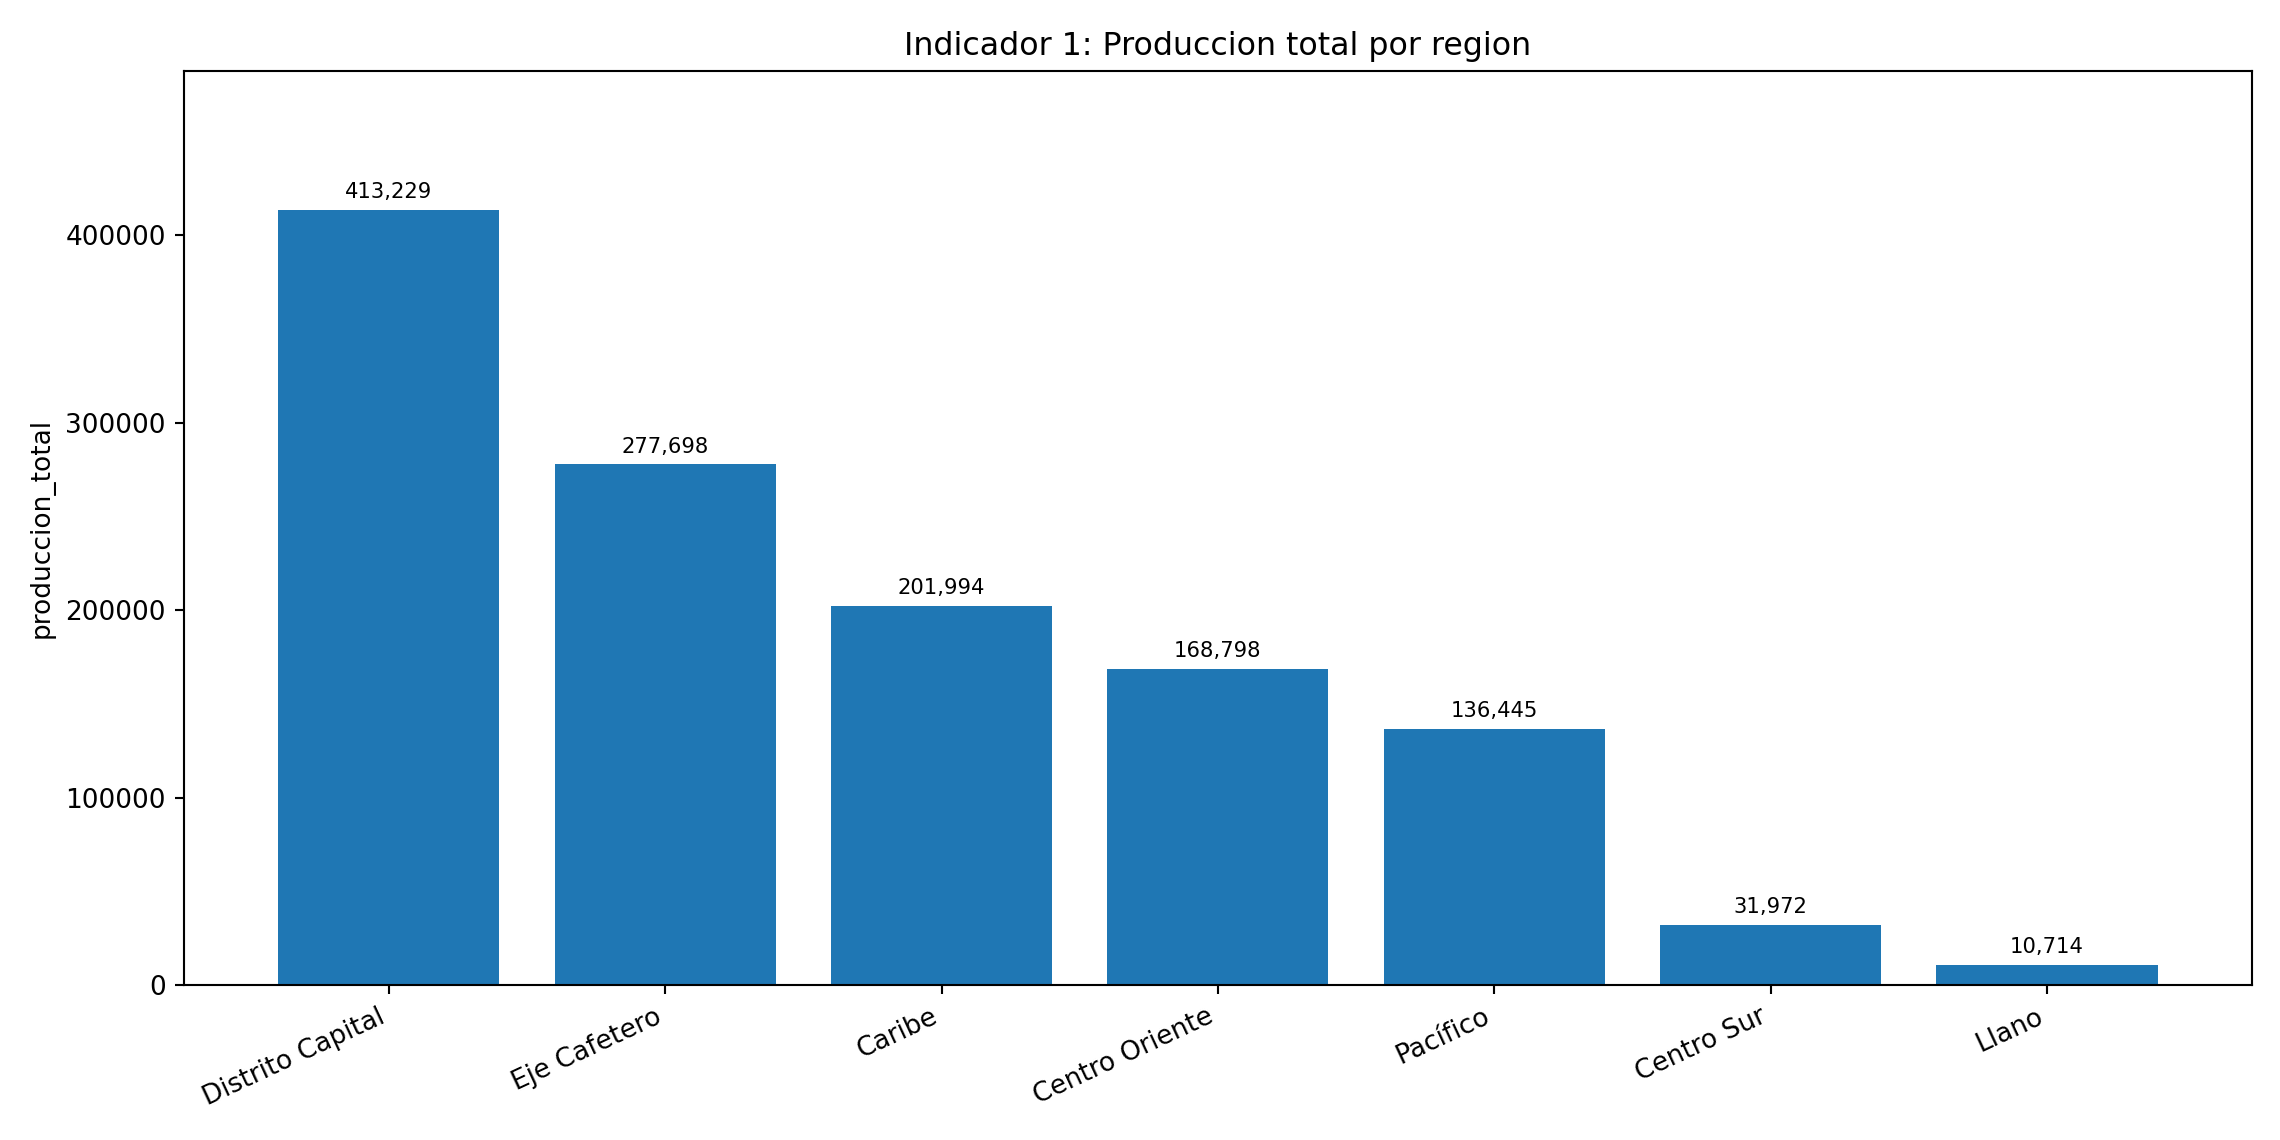
\includegraphics[width=0.92\textwidth]{indicadores/indicador_01.png}
\caption{Indicador 1. Produccion total por region.}
\end{figure}

\begin{longtable}{rrlr}
\caption{Indicador 1. Produccion total por region: tabla por convocatoria.} \label{tab:ind01_conv} \\
\toprule
ID\_CONVOCATORIA & ANIO\_CONVOCATORIA & NME\_REGION\_GR & produccion\_total \\
\midrule
\endfirsthead
\caption[]{Indicador 1. Produccion total por region: tabla por convocatoria.} \\
\toprule
ID\_CONVOCATORIA & ANIO\_CONVOCATORIA & NME\_REGION\_GR & produccion\_total \\
\midrule
\endhead
\midrule
\multicolumn{4}{r}{Continued on next page} \\
\midrule
\endfoot
\bottomrule
\endlastfoot
19 & 2017 & Distrito Capital & 99521 \\
19 & 2017 & Eje Cafetero & 57701 \\
19 & 2017 & Caribe & 40852 \\
19 & 2017 & Centro Oriente & 34380 \\
19 & 2017 & Pacífico & 31792 \\
19 & 2017 & Centro Sur & 5953 \\
19 & 2017 & Llano & 1725 \\
20 & 2019 & Distrito Capital & 144937 \\
20 & 2019 & Eje Cafetero & 102664 \\
20 & 2019 & Caribe & 75971 \\
20 & 2019 & Centro Oriente & 57967 \\
20 & 2019 & Pacífico & 47916 \\
20 & 2019 & Centro Sur & 10863 \\
20 & 2019 & Llano & 4130 \\
21 & 2021 & Distrito Capital & 168771 \\
21 & 2021 & Eje Cafetero & 117333 \\
21 & 2021 & Caribe & 85171 \\
21 & 2021 & Centro Oriente & 76451 \\
21 & 2021 & Pacífico & 56737 \\
21 & 2021 & Centro Sur & 15156 \\
21 & 2021 & Llano & 4859 \\
\end{longtable}


\textbf{Analisis concreto.} El volumen de produccion esta fuertemente concentrado en Distrito Capital, con 413229 registros, seguido por Eje Cafetero (277698) y Caribe (201994). En el extremo inferior aparece Llano con 10714 productos, lo que confirma una distribucion territorial altamente asimetrica y una brecha estructural entre las regiones lideres y las regiones perifericas.



\subsection{Indicador 2. Participacion regional}
\textbf{Formula:}
\[
\%_r = \left(\frac{P_r}{P_t}\right) \times 100
\]
\textbf{Para que se utiliza:} comparar el peso relativo de cada region en el total nacional.



\renewcommand{\arraystretch}{1.5}
\setlength{\LTleft}{0pt}
\setlength{\LTright}{0pt}

\small

\begin{center}

\begin{longtable}{cccrrr}

\caption{Indicador 2. Participación regional (\%) por convocatoria}
\label{tab:ind02_conv} \\

\toprule

\textbf{ID} &
\textbf{Año} &
\textbf{Región} &
\textbf{Producción} &
\textbf{Total nacional} &
\textbf{Participación (\%)} \\

\midrule
\endfirsthead

\caption[]{Indicador 2. Participación regional (\%) por convocatoria -- continuación} \\

\toprule

\textbf{ID} &
\textbf{Año} &
\textbf{Región} &
\textbf{Producción} &
\textbf{Total nacional} &
\textbf{Participación (\%)} \\

\midrule
\endhead

\midrule
\multicolumn{6}{r}{Continúa en la siguiente página} \\
\midrule
\endfoot

\bottomrule
\endlastfoot


19 & 2017 & Distrito Capital & 99521 & 271924 & 36.5988 \\
19 & 2017 & Eje Cafetero & 57701 & 271924 & 21.2195 \\
19 & 2017 & Caribe & 40852 & 271924 & 15.0233 \\
19 & 2017 & Centro Oriente & 34380 & 271924 & 12.6432 \\
19 & 2017 & Pacífico & 31792 & 271924 & 11.6915 \\
19 & 2017 & Centro Sur & 5953 & 271924 & 2.1892 \\
19 & 2017 & Llano & 1725 & 271924 & 0.6344 \\

20 & 2019 & Distrito Capital & 144937 & 444448 & 32.6106 \\
20 & 2019 & Eje Cafetero & 102664 & 444448 & 23.0992 \\
20 & 2019 & Caribe & 75971 & 444448 & 17.0933 \\
20 & 2019 & Centro Oriente & 57967 & 444448 & 13.0425 \\
20 & 2019 & Pacífico & 47916 & 444448 & 10.7810 \\
20 & 2019 & Centro Sur & 10863 & 444448 & 2.4442 \\
20 & 2019 & Llano & 4130 & 444448 & 0.9292 \\

21 & 2021 & Distrito Capital & 168771 & 524478 & 32.1789 \\
21 & 2021 & Eje Cafetero & 117333 & 524478 & 22.3714 \\
21 & 2021 & Caribe & 85171 & 524478 & 16.2392 \\
21 & 2021 & Centro Oriente & 76451 & 524478 & 14.5766 \\
21 & 2021 & Pacífico & 56737 & 524478 & 10.8178 \\
21 & 2021 & Centro Sur & 15156 & 524478 & 2.8897 \\
21 & 2021 & Llano & 4859 & 524478 & 0.9264 \\

\end{longtable}

\end{center}

\begin{figure}[H]
\centering
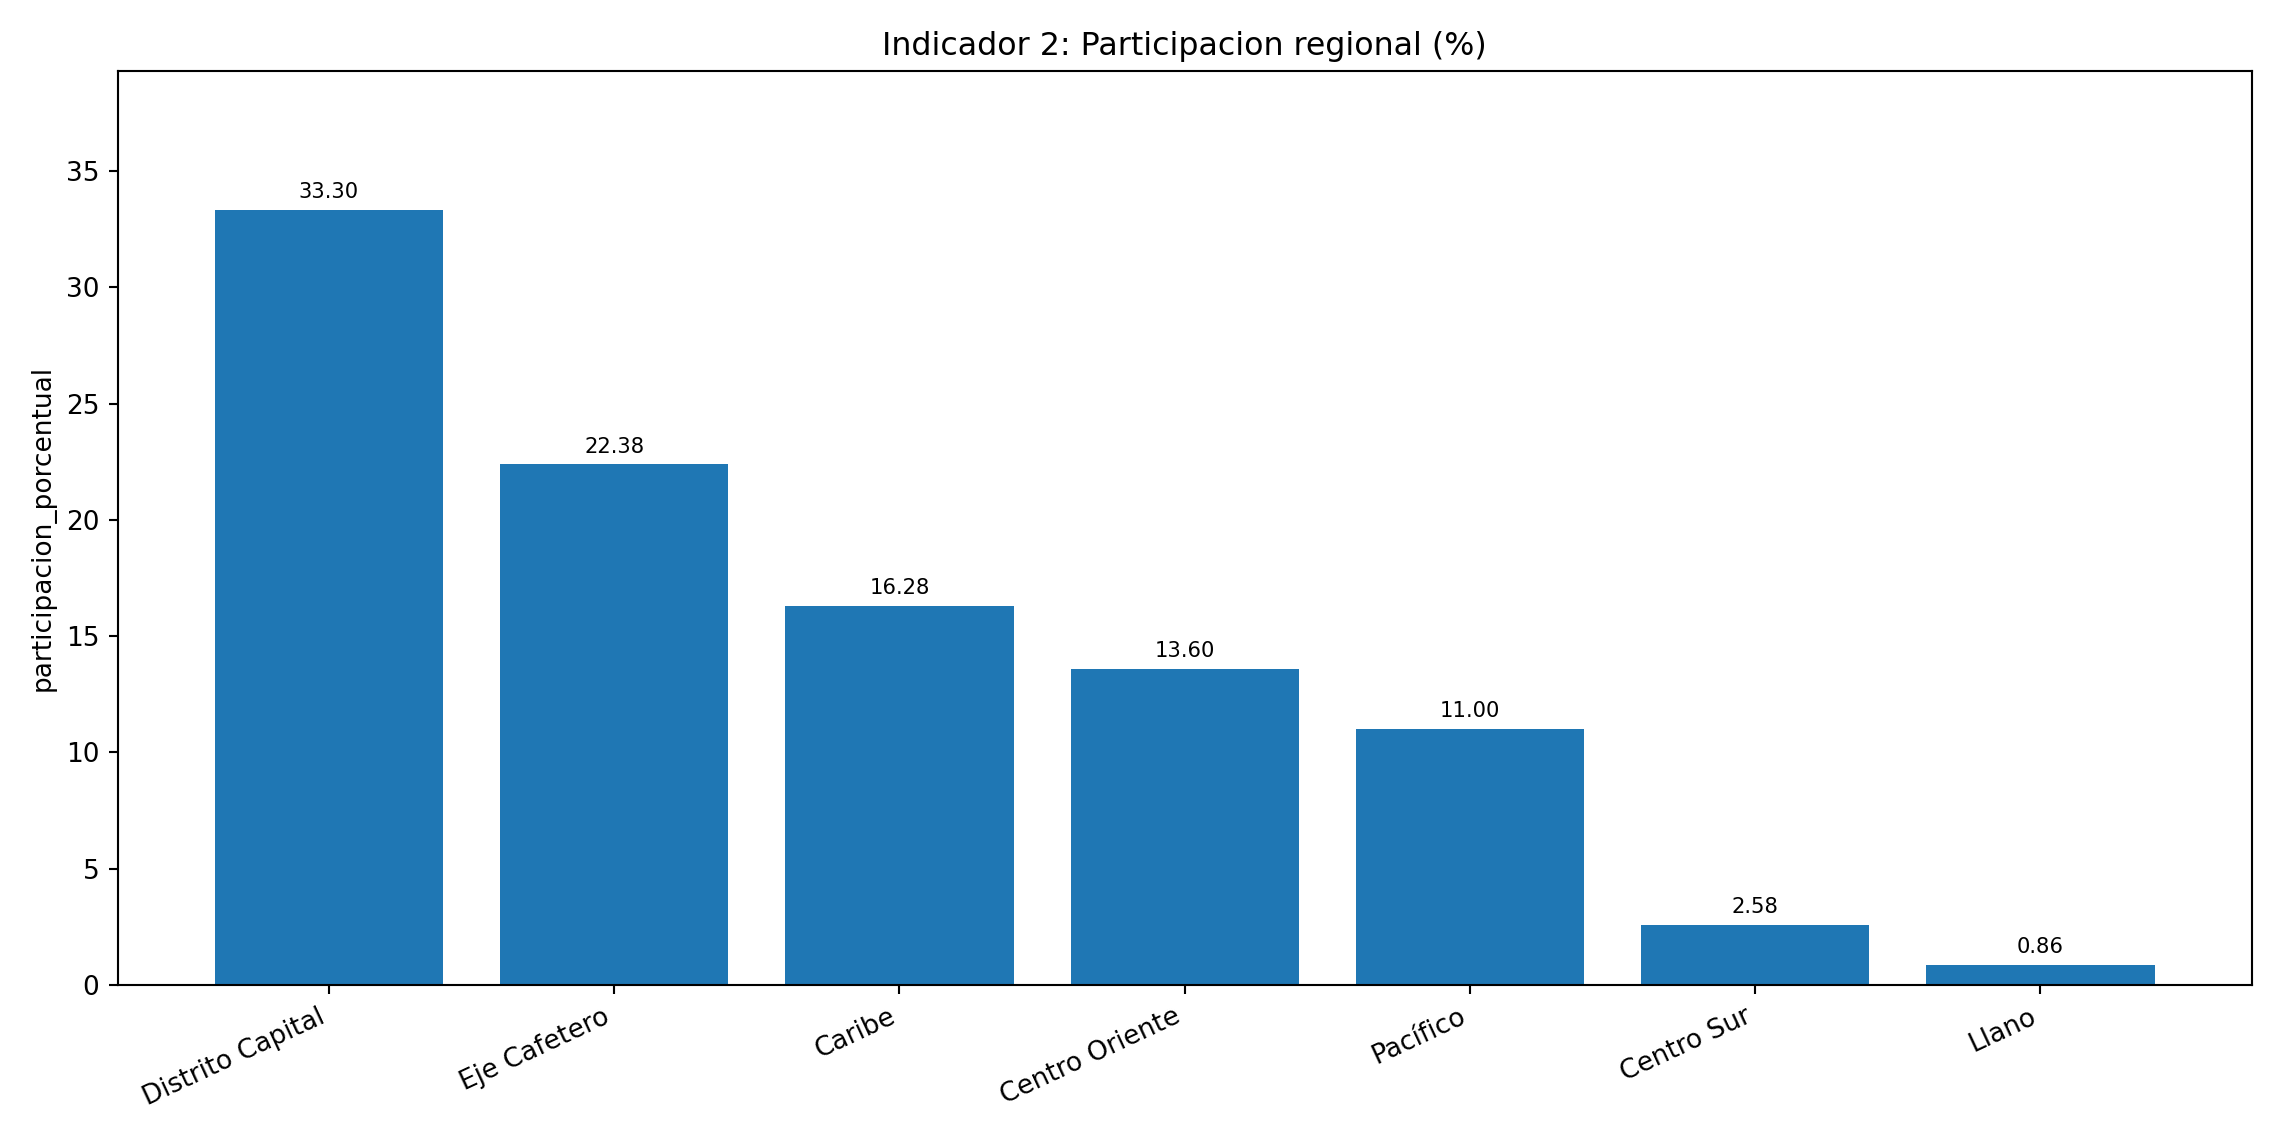
\includegraphics[width=0.92\textwidth]{indicadores/indicador_02.png}

\caption{Indicador 2. Participacion regional.}
\end{figure}
\textbf{Analisis concreto.} La participacion regional confirma el liderazgo de Distrito Capital con 33.3021\% de la produccion nacional, muy por encima de Eje Cafetero (22.3797\%) y Caribe (16.2787\%). Llano registra apenas 0.8634\%, por lo que su peso relativo en el sistema nacional es marginal. Este indicador permite leer la concentracion de la produccion en terminos proporcionales y no solo absolutos.



\subsection{Indicador 3. Produccion promedio por grupo}
\textbf{Formula:}
\[
Prom_r = \frac{P_r}{G_r}
\]
\textbf{Para que se utiliza:} medir la intensidad promedio de produccion por grupo en cada region.

\begin{longtable}{lrrr}
\caption{Indicador 3. Produccion promedio por grupo: tabla completa.} \label{tab:ind03_general} \\
\toprule
NME\_REGION\_GR & produccion\_total & grupos\_unicos & produccion\_promedio\_por\_grupo \\
\midrule
\endfirsthead
\caption[]{Indicador 3. Produccion promedio por grupo: tabla completa.} \\
\toprule
NME\_REGION\_GR & produccion\_total & grupos\_unicos & produccion\_promedio\_por\_grupo \\
\midrule
\endhead
\midrule
\multicolumn{4}{r}{Continued on next page} \\
\midrule
\endfoot
\bottomrule
\endlastfoot
Caribe & 201994 & 859 & 235.1502 \\
Eje Cafetero & 277698 & 1327 & 209.2675 \\
Centro Oriente & 168798 & 838 & 201.4296 \\
Distrito Capital & 413229 & 2163 & 191.0444 \\
Pacífico & 136445 & 765 & 178.3595 \\
Centro Sur & 31972 & 241 & 132.6639 \\
Llano & 10714 & 111 & 96.5225 \\
\end{longtable}

\renewcommand{\arraystretch}{1.3}
\setlength{\LTleft}{0pt}
\setlength{\LTright}{0pt}

\small

\begin{center}

\begin{longtable}{cccrrr}

\caption{Indicador 3. Producción promedio por grupo por convocatoria}
\label{tab:ind03_conv} \\

\toprule

\textbf{ID  }   &
\textbf{Año  }   &
\textbf{Región }   &
\textbf{Producción  }   &
\textbf{Grupo }   &
\textbf{Promedio por grupo  } \\

\midrule
\endfirsthead

\caption[]{Indicador 3. Producción promedio por grupo por convocatoria -- continuación} \\

\toprule

\textbf{ID }  &
\textbf{Año }  &
\textbf{Región }   &
\textbf{Producción }  &
\textbf{Grupos }  &
\textbf{Promedio por grupo  } \\

\midrule
\endhead

\midrule
\multicolumn{6}{r}{Continúa en la siguiente página} \\
\midrule
\endfoot

\bottomrule
\endlastfoot


19   &  2017 &  Caribe  &  40852 &  620 & 65.8903  \\
19 & 2017 & Distrito Capital  & 99521 & 1628 & 61.1308  \\
19 & 2017 & Pacífico  & 31792  & 526 & 60.4411  \\
19 & 2017 & Centro Oriente  & 34380 & 569 & 60.4218  \\
19 & 2017 & Eje Cafetero  & 57701 & 977 & 59.0594 \\
19 & 2017 & Centro Sur  & 5953 & 154 & 38.6558 \\
19 & 2017 & Llano & 1725 & 55 & 31.3636 \\

20 & 2019 & Caribe & 75971 & 751 & 101.1598 \\
20 & 2019 & Eje Cafetero & 102664 & 1175 & 87.3736 \\
20 & 2019 & Centro Oriente & 57967 & 703 & 82.4566 \\
20 & 2019 & Distrito Capital & 144937 & 1765 & 82.1173 \\
20 & 2019 & Pacífico & 47916 & 636 & 75.3396 \\
20 & 2019 & Centro Sur & 10863 & 188 & 57.7819 \\
20 & 2019 & Llano & 4130 & 83 & 49.7590 \\

21 & 2021 & Caribe & 85171 & 810 & 105.1494 \\
21 & 2021 & Centro Oriente & 76451 & 775 & 98.6465 \\
21 & 2021 & Eje Cafetero & 117333 & 1206 & 97.2910 \\
21 & 2021 & Distrito Capital & 168771 & 1855 & 90.9817 \\
21 & 2021 & Pacífico & 56737 & 688 & 82.4666 \\
21 & 2021 & Centro Sur & 15156 & 210 & 72.1714 \\
21 & 2021 & Llano & 4859 & 93 & 52.2473 \\

\end{longtable}

\end{center}

\begin{figure}[H]
\centering
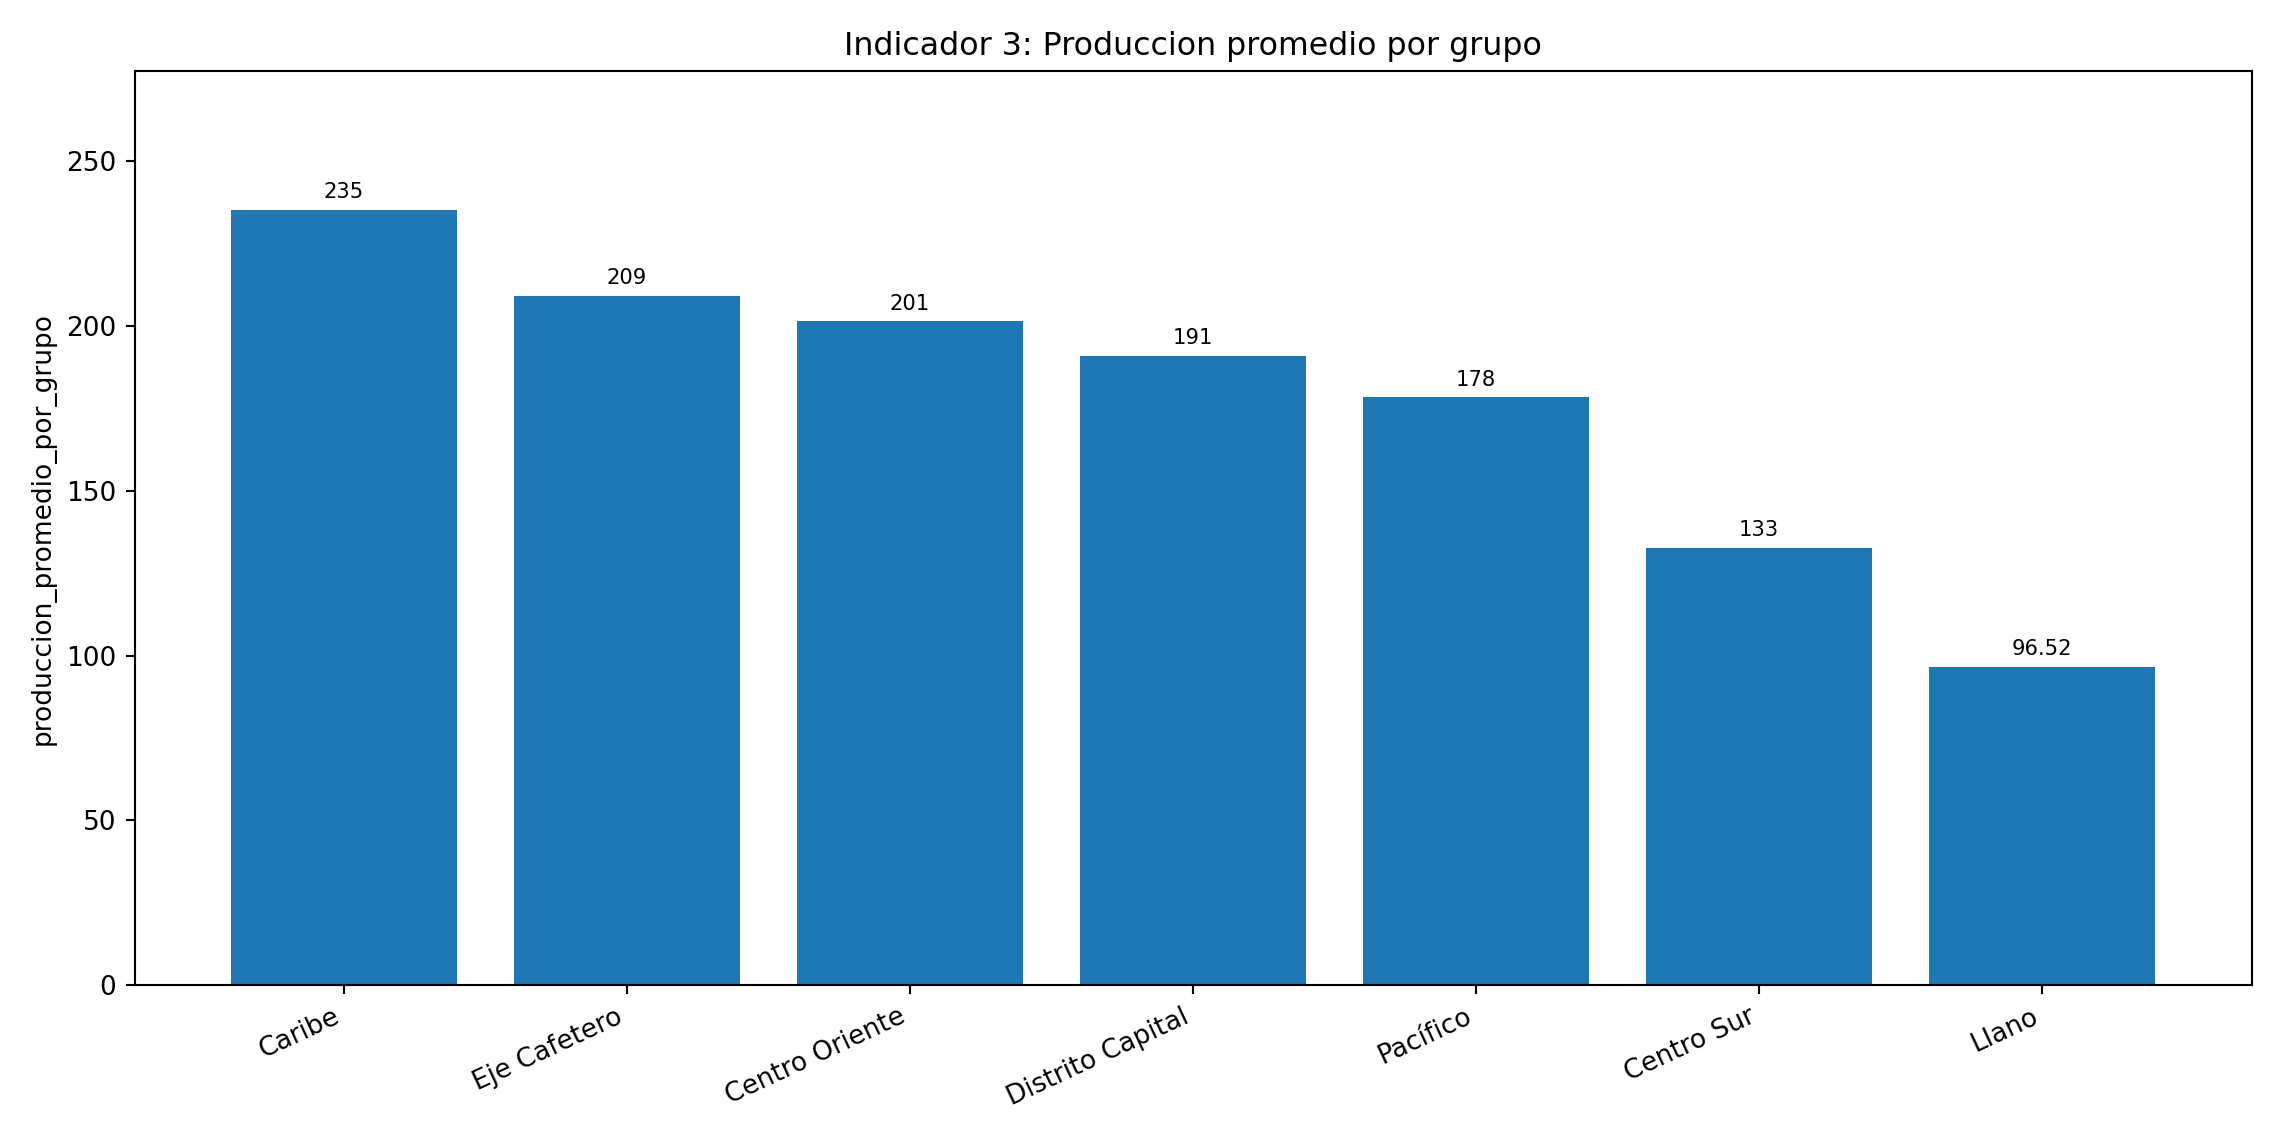
\includegraphics[width=0.92\textwidth]{indicadores/indicador_03.png}
\caption{Indicador 3. Produccion promedio por grupo.}
\end{figure}

\textbf{Analisis concreto.} Caribe presenta el promedio mas alto de produccion por grupo (235.1502), seguido por Eje Cafetero (209.2675) y Centro Oriente (201.4296). Llano exhibe el menor valor (96.5225), lo que indica menor intensidad productiva promedio por unidad de analisis. La lectura estadistica sugiere que algunas regiones producen menos en volumen total, pero sostienen mayor eficiencia media por grupo.


\subsection{Indicador 4. Produccion por clasificacion del grupo}
\textbf{Formula:}
\[
P_{r,c} = \text{productos en region } r \text{ para clasificacion } c
\]
\textbf{Para que se utiliza:} analizar la composicion de la produccion por nivel de clasificacion de grupos.

\input{tablas_indicadores/indicador_04_tabla_general.tex}




\renewcommand{\arraystretch}{1.2}
\setlength{\LTleft}{0pt}
\setlength{\LTright}{0pt}

\small

\begin{center}

\begin{longtable}{ccllr}

\caption{Indicador 4. Producción por clasificación por convocatoria}
\label{tab:ind04_conv} \\

\toprule

\textbf{ID} &
\textbf{Año} &
\textbf{Región} &
\textbf{Clasificación} &
\textbf{Productos} \\

\midrule
\endfirsthead

\caption[]{Indicador 4. Producción por clasificación por convocatoria} \\

\toprule

\textbf{ID} &
\textbf{Año} &
\textbf{Región} &
\textbf{Clasificación} &
\textbf{Productos} \\

\midrule
\endhead

\midrule
\multicolumn{5}{r}{Continúa en la siguiente página} \\
\midrule
\endfoot

\bottomrule
\endlastfoot


19 & 2017 & Caribe & A & 12864 \\
19 & 2017 & Caribe & A1 & 8510 \\
19 & 2017 & Caribe & B & 10471 \\
19 & 2017 & Caribe & C & 8264 \\
19 & 2017 & Caribe & Reconocido & 743 \\

19 & 2017 & Centro Oriente & A & 7739 \\
19 & 2017 & Centro Oriente & A1 & 5351 \\
19 & 2017 & Centro Oriente & B & 10738 \\
19 & 2017 & Centro Oriente & C & 8877 \\
19 & 2017 & Centro Oriente & Reconocido & 1675 \\

19 & 2017 & Centro Sur & A & 1091 \\
19 & 2017 & Centro Sur & A1 & 620 \\
19 & 2017 & Centro Sur & B & 1795 \\
19 & 2017 & Centro Sur & C & 1951 \\
19 & 2017 & Centro Sur & Reconocido & 496 \\

19 & 2017 & Distrito Capital & A & 20783 \\
19 & 2017 & Distrito Capital & A1 & 26289 \\
19 & 2017 & Distrito Capital & B & 26502 \\
19 & 2017 & Distrito Capital & C & 22314 \\
19 & 2017 & Distrito Capital & Reconocido & 3633 \\

19 & 2017 & Eje Cafetero & A & 12867 \\
19 & 2017 & Eje Cafetero & A1 & 16782 \\
19 & 2017 & Eje Cafetero & B & 15914 \\
19 & 2017 & Eje Cafetero & C & 10057 \\
19 & 2017 & Eje Cafetero & Reconocido & 2081 \\

19 & 2017 & Llano & A & 162 \\
19 & 2017 & Llano & B & 385 \\
19 & 2017 & Llano & C & 1035 \\
19 & 2017 & Llano & Reconocido & 143 \\

19 & 2017 & Pacífico & A & 6240 \\
19 & 2017 & Pacífico & A1 & 8781 \\
19 & 2017 & Pacífico & B & 9194 \\
19 & 2017 & Pacífico & C & 6896 \\
19 & 2017 & Pacífico & Reconocido & 681 \\

20 & 2019 & Caribe & A & 24318 \\
20 & 2019 & Caribe & A1 & 19748 \\
20 & 2019 & Caribe & B & 19664 \\
20 & 2019 & Caribe & C & 11494 \\
20 & 2019 & Caribe & Reconocido & 747 \\

20 & 2019 & Centro Oriente & A & 16672 \\
20 & 2019 & Centro Oriente & A1 & 9976 \\
20 & 2019 & Centro Oriente & B & 16965 \\
20 & 2019 & Centro Oriente & C & 13767 \\
20 & 2019 & Centro Oriente & Reconocido & 587 \\

20 & 2019 & Centro Sur & A & 2221 \\
20 & 2019 & Centro Sur & A1 & 1517 \\
20 & 2019 & Centro Sur & B & 3782 \\
20 & 2019 & Centro Sur & C & 2944 \\
20 & 2019 & Centro Sur & Reconocido & 399 \\

20 & 2019 & Distrito Capital & A & 35471 \\
20 & 2019 & Distrito Capital & A1 & 44078 \\
20 & 2019 & Distrito Capital & B & 35996 \\
20 & 2019 & Distrito Capital & C & 25723 \\
20 & 2019 & Distrito Capital & Reconocido & 3669 \\

20 & 2019 & Eje Cafetero & A & 26375 \\
20 & 2019 & Eje Cafetero & A1 & 36443 \\
20 & 2019 & Eje Cafetero & B & 22090 \\
20 & 2019 & Eje Cafetero & C & 16488 \\
20 & 2019 & Eje Cafetero & Reconocido & 1268 \\

20 & 2019 & Llano & A & 549 \\
20 & 2019 & Llano & A1 & 90 \\
20 & 2019 & Llano & B & 1055 \\
20 & 2019 & Llano & C & 2392 \\
20 & 2019 & Llano & Reconocido & 44 \\

20 & 2019 & Pacífico & A & 12615 \\
20 & 2019 & Pacífico & A1 & 12060 \\
20 & 2019 & Pacífico & B & 11829 \\
20 & 2019 & Pacífico & C & 10471 \\
20 & 2019 & Pacífico & Reconocido & 941 \\

21 & 2021 & Caribe & A & 27165 \\
21 & 2021 & Caribe & A1 & 24155 \\
21 & 2021 & Caribe & B & 18772 \\
21 & 2021 & Caribe & C & 12650 \\
21 & 2021 & Caribe & Reconocido & 2429 \\

21 & 2021 & Centro Oriente & A & 24602 \\
21 & 2021 & Centro Oriente & A1 & 13348 \\
21 & 2021 & Centro Oriente & B & 21007 \\
21 & 2021 & Centro Oriente & C & 16266 \\
21 & 2021 & Centro Oriente & Reconocido & 1228 \\

21 & 2021 & Centro Sur & A & 4267 \\
21 & 2021 & Centro Sur & A1 & 2138 \\
21 & 2021 & Centro Sur & B & 4187 \\
21 & 2021 & Centro Sur & C & 3814 \\
21 & 2021 & Centro Sur & Reconocido & 750 \\

21 & 2021 & Distrito Capital & A & 41802 \\
21 & 2021 & Distrito Capital & A1 & 58122 \\
21 & 2021 & Distrito Capital & B & 38398 \\
21 & 2021 & Distrito Capital & C & 27415 \\
21 & 2021 & Distrito Capital & Reconocido & 3034 \\

21 & 2021 & Eje Cafetero & A & 34699 \\
21 & 2021 & Eje Cafetero & A1 & 44109 \\
21 & 2021 & Eje Cafetero & B & 21984 \\
21 & 2021 & Eje Cafetero & C & 14963 \\
21 & 2021 & Eje Cafetero & Reconocido & 1578 \\

21 & 2021 & Llano & A & 479 \\
21 & 2021 & Llano & A1 & 357 \\
21 & 2021 & Llano & B & 1908 \\
21 & 2021 & Llano & C & 2000 \\
21 & 2021 & Llano & Reconocido & 115 \\

21 & 2021 & Pacífico & A & 14933 \\
21 & 2021 & Pacífico & A1 & 15226 \\
21 & 2021 & Pacífico & B & 12683 \\
21 & 2021 & Pacífico & C & 12540 \\
21 & 2021 & Pacífico & Reconocido & 1355 \\

\end{longtable}

\end{center}

\begin{figure}[H]
\centering
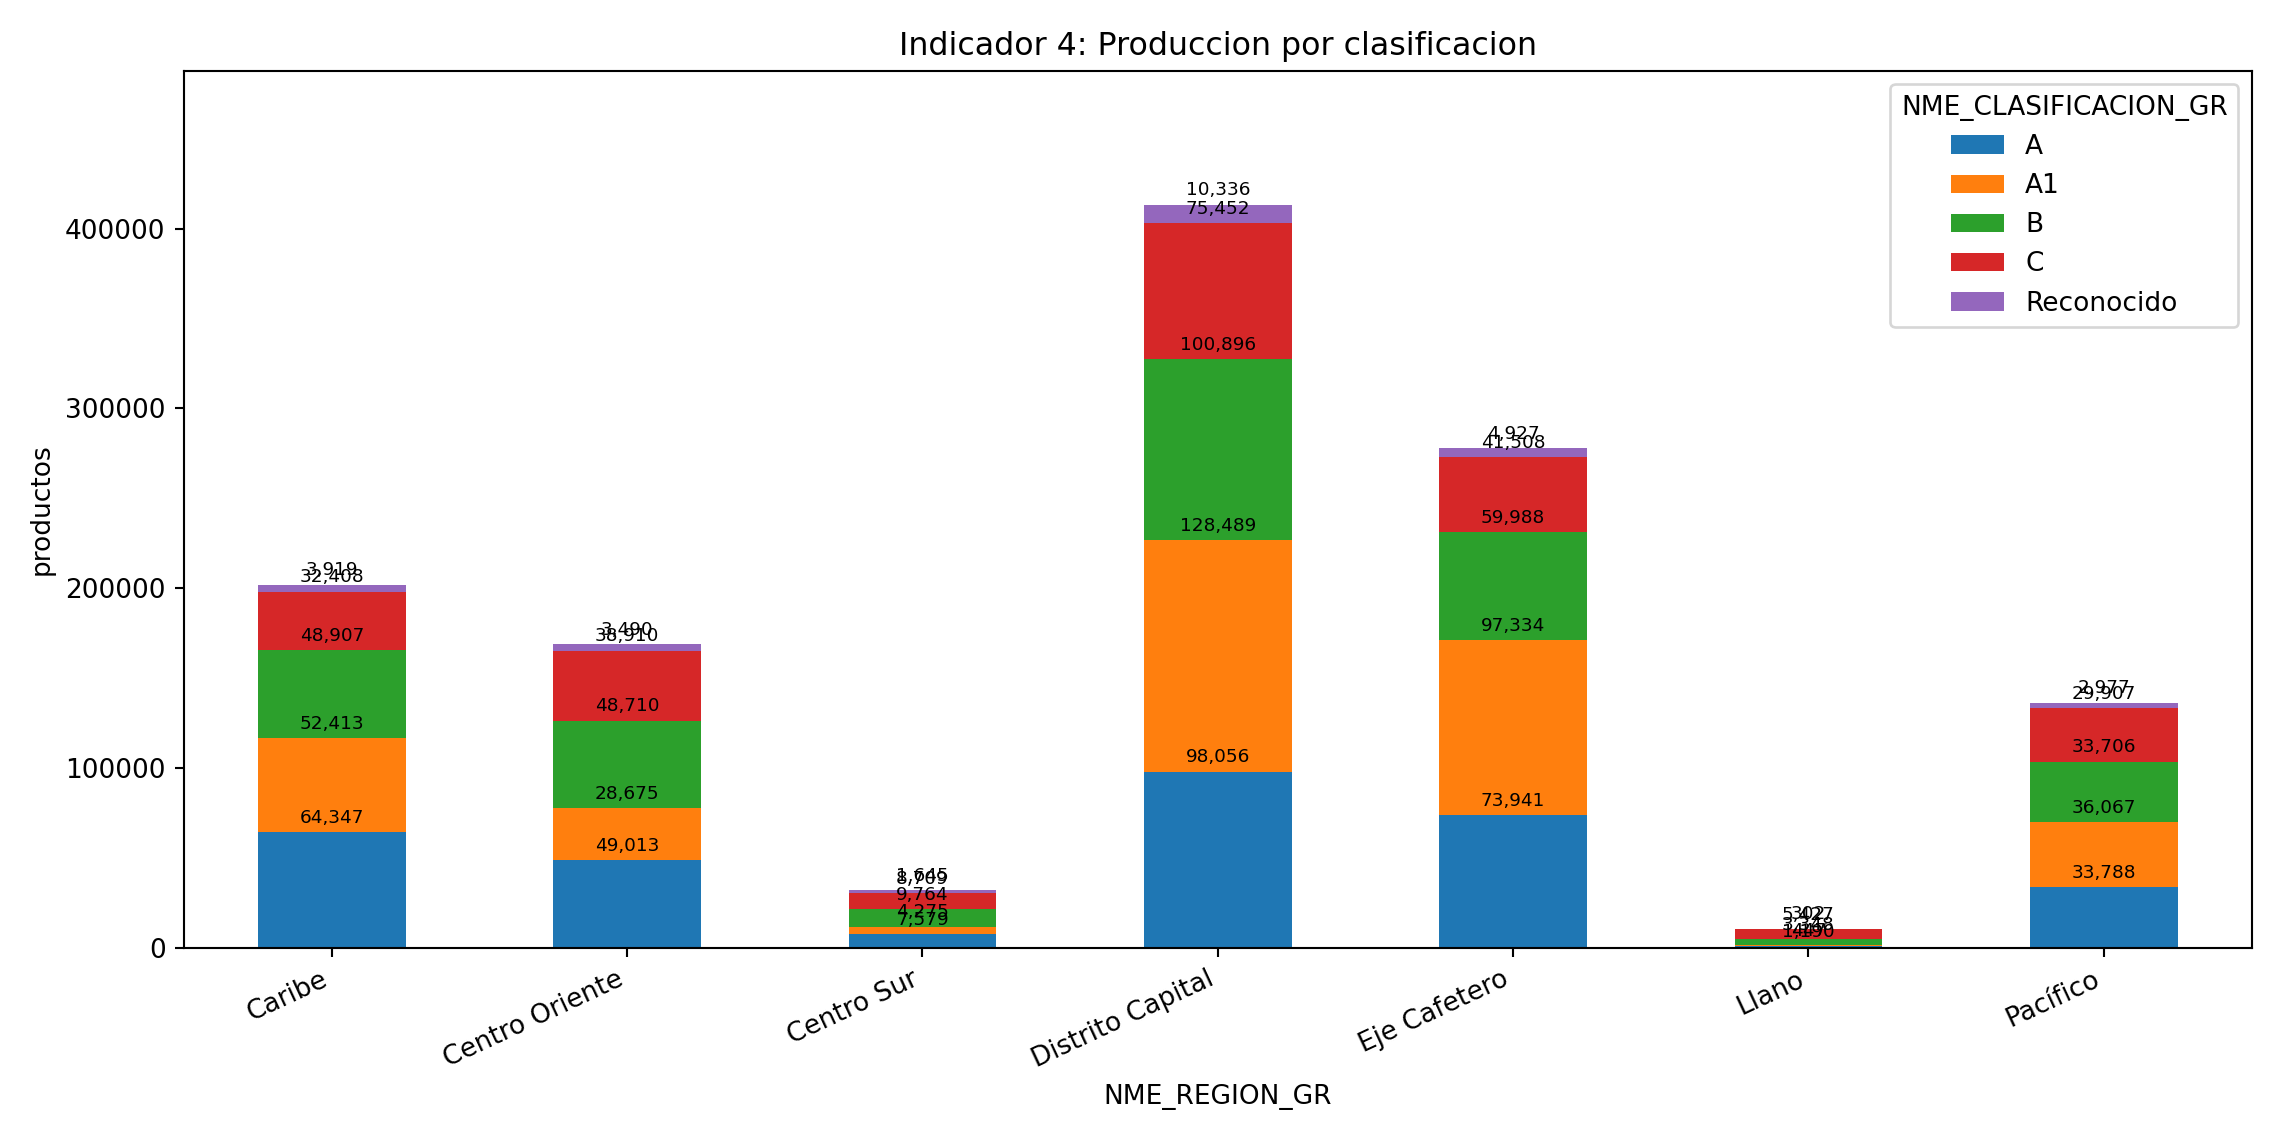
\includegraphics[width=0.92\textwidth]{indicadores/indicador_04.png}
\caption{Indicador 4. Produccion por clasificacion del grupo.}
\end{figure}


\textbf{Analisis concreto.} La produccion por clasificacion se concentra principalmente en A1 (347700 productos) y A (327914), seguidas por B (305319) y C (232321). A nivel territorial, Distrito Capital lidera en todas las clasificaciones con 413229 productos totales, y el mayor valor puntual se observa en su categoria A1 (128489). Esto indica que la mayor parte del volumen se sostiene en grupos clasificados en niveles altos de desempeno.


\subsection{Indicador 5. Diversificacion de productos}
\textbf{Formula:}
\[
D_r = |T_r|
\]
\textbf{Para que se utiliza:} medir variedad de tipologias de productos por region.

\begin{longtable}{lrr}
\caption{Indicador 5. Diversificacion de productos: tabla completa.} \label{tab:ind05_general} \\
\toprule
NME\_REGION\_GR & tipologias\_distintas & productos\_considerados \\
\midrule
\endfirsthead
\caption[]{Indicador 5. Diversificacion de productos: tabla completa.} \\
\toprule
NME\_REGION\_GR & tipologias\_distintas & productos\_considerados \\
\midrule
\endhead
\midrule
\multicolumn{3}{r}{Continued on next page} \\
\midrule
\endfoot
\bottomrule
\endlastfoot
Distrito Capital & 75 & 413229 \\
Eje Cafetero & 74 & 277698 \\
Centro Oriente & 71 & 168798 \\
Pacífico & 71 & 136445 \\
Caribe & 70 & 201994 \\
Centro Sur & 66 & 31972 \\
Llano & 59 & 10714 \\
\end{longtable}


\renewcommand{\arraystretch}{1.2}
\setlength{\LTleft}{0pt}
\setlength{\LTright}{0pt}

\small

\begin{center}

\begin{longtable}{cclrr}

\caption{Indicador 5. Diversificación de productos por convocatoria}
\label{tab:ind05_conv} \\

\toprule

\textbf{ID} &
\textbf{Año} &
\textbf{Región} &
\textbf{Tipologías distintas} &
\textbf{Productos considerados} \\

\midrule
\endfirsthead

\caption[]{Indicador 5. Diversificación de productos por convocatoria -- continuación} \\

\toprule

\textbf{ID} &
\textbf{Año} &
\textbf{Región} &
\textbf{Tipologías distintas} &
\textbf{Productos considerados} \\

\midrule
\endhead

\midrule
\multicolumn{5}{r}{Continúa en la siguiente página} \\
\midrule
\endfoot

\bottomrule
\endlastfoot


19 & 2017 & Distrito Capital & 52 & 99521 \\
19 & 2017 & Caribe & 51 & 40852 \\
19 & 2017 & Eje Cafetero & 51 & 57701 \\
19 & 2017 & Centro Oriente & 50 & 34380 \\
19 & 2017 & Pacífico & 47 & 31792 \\
19 & 2017 & Centro Sur & 41 & 5953 \\
19 & 2017 & Llano & 33 & 1725 \\

20 & 2019 & Distrito Capital & 62 & 144937 \\
20 & 2019 & Eje Cafetero & 61 & 102664 \\
20 & 2019 & Caribe & 58 & 75971 \\
20 & 2019 & Centro Oriente & 58 & 57967 \\
20 & 2019 & Pacífico & 58 & 47916 \\
20 & 2019 & Centro Sur & 52 & 10863 \\
20 & 2019 & Llano & 49 & 4130 \\

21 & 2021 & Distrito Capital & 62 & 168771 \\
21 & 2021 & Eje Cafetero & 62 & 117333 \\
21 & 2021 & Pacífico & 60 & 56737 \\
21 & 2021 & Caribe & 59 & 85171 \\
21 & 2021 & Centro Oriente & 59 & 76451 \\
21 & 2021 & Centro Sur & 54 & 15156 \\
21 & 2021 & Llano & 44 & 4859 \\

\end{longtable}

\end{center}

\begin{figure}[H]
\centering
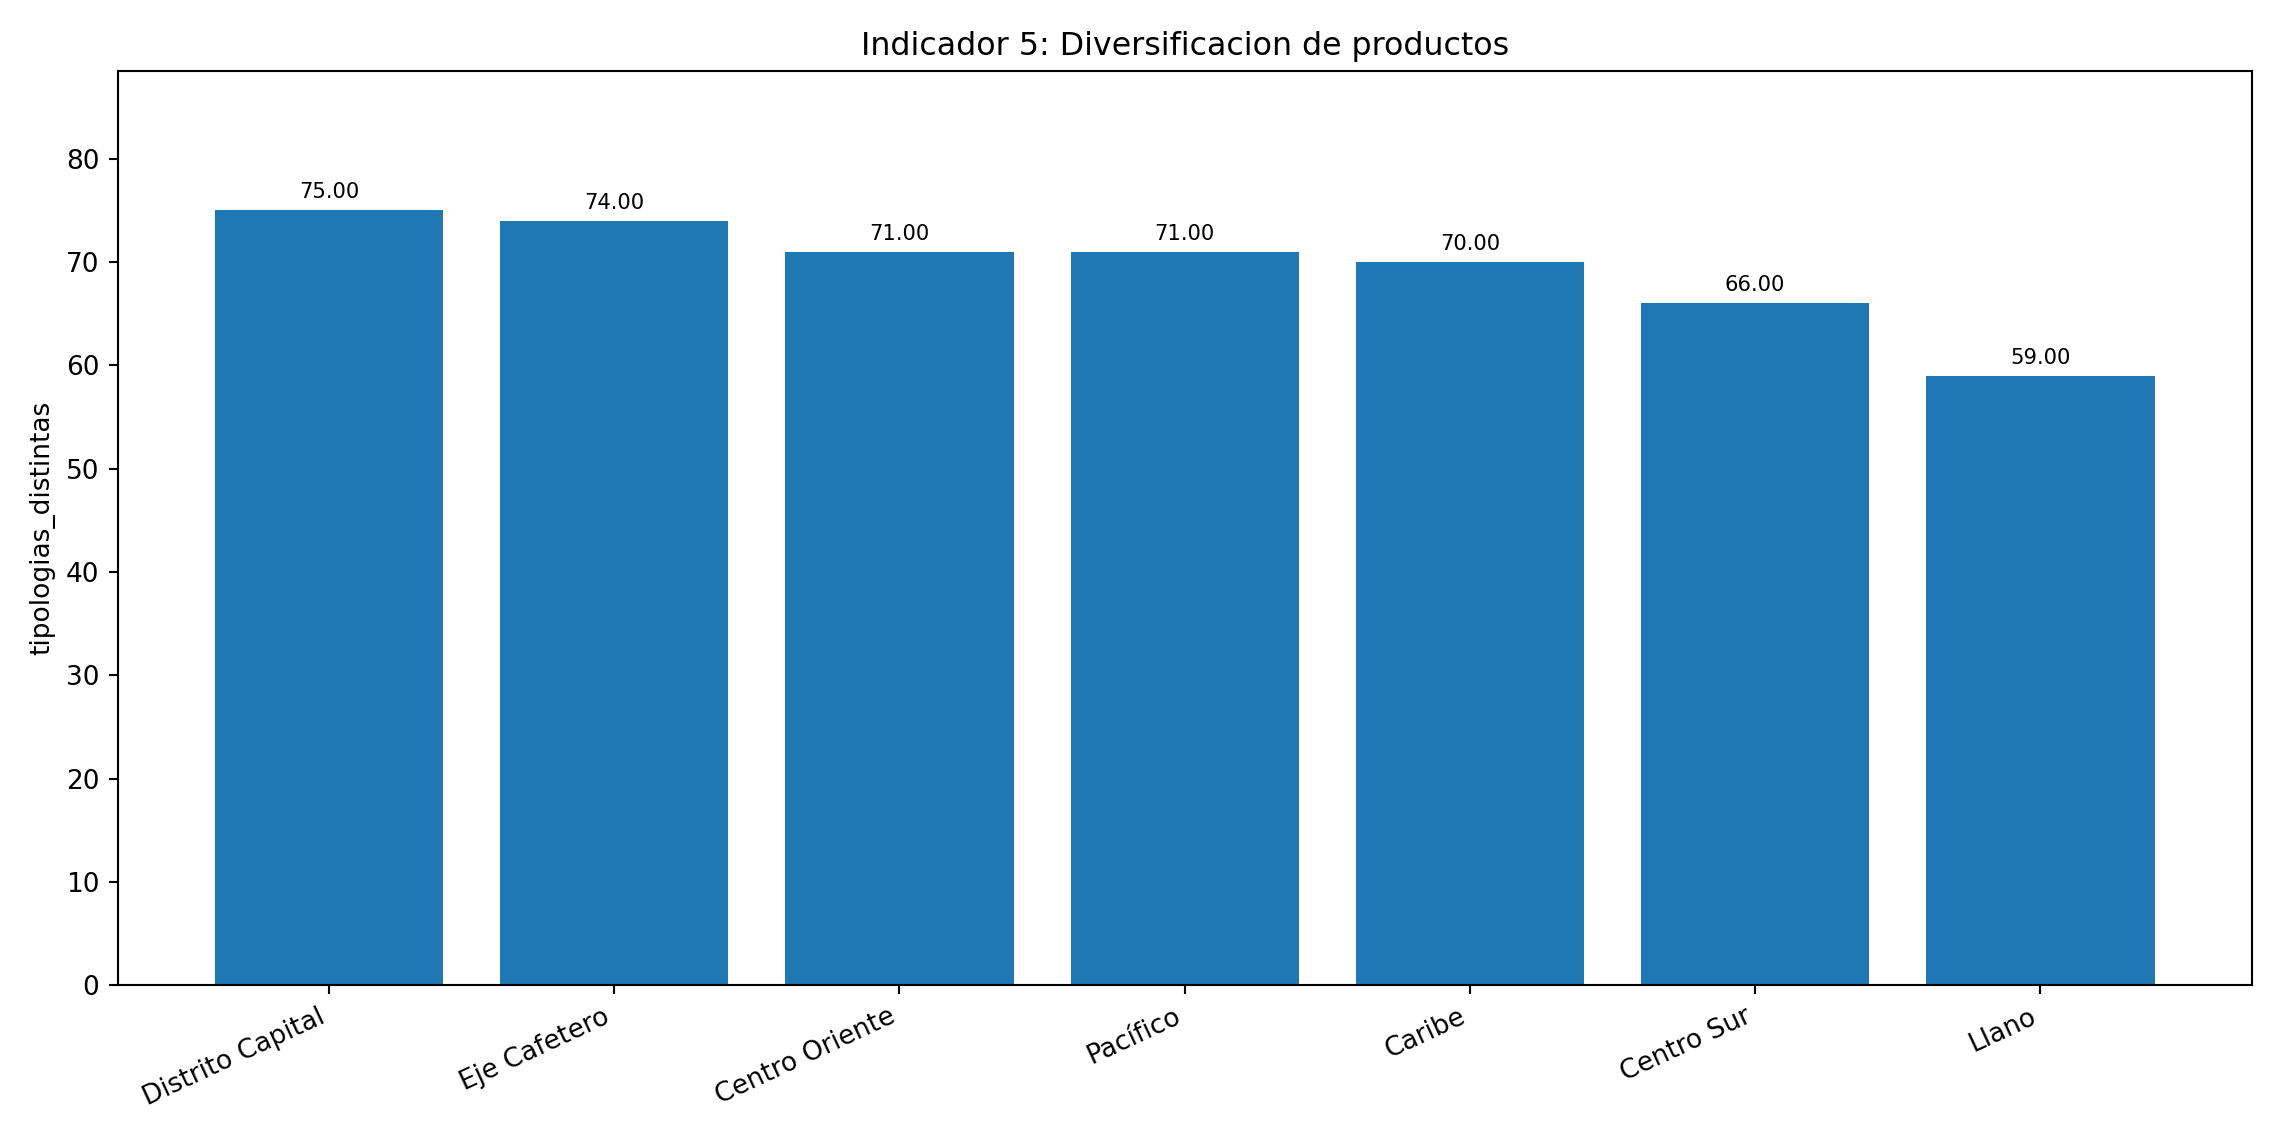
\includegraphics[width=0.92\textwidth]{indicadores/indicador_05.png}
\caption{Indicador 5. Diversificacion de productos.}
\end{figure}

\textbf{Analisis concreto.} La diversificacion de productos es mayor en Distrito Capital, con 75 tipologias distintas, seguido por Eje Cafetero con 74. Llano registra 59 tipologias, el valor mas bajo del conjunto. En terminos comparativos, la diferencia entre el maximo y el minimo es de 16 tipologias, lo que evidencia heterogeneidad en la amplitud del portafolio cientifico regional.


\subsection{Indicador 6. Indice de especializacion productiva}
\textbf{Formula:}
\[
IEP_r = \frac{\text{participacion de productos}_r}{\text{participacion de grupos}_r}
\]
\textbf{Para que se utiliza:} evaluar si la region produce proporcionalmente por encima o por debajo de su peso en grupos.

\begin{longtable}{lrrrrr}
\caption{Indicador 6. Indice de especializacion productiva: tabla completa.} \label{tab:ind06_general} \\
\toprule
NME\_REGION\_GR & productos & grupos\_unicos & participacion\_productos & participacion\_grupos & indice\_especializacion\_productiva \\
\midrule
\endfirsthead
\caption[]{Indicador 6. Indice de especializacion productiva: tabla completa.} \\
\toprule
NME\_REGION \_GR & productos & grupos\_unicos & participacion\_productos & participacion\_grupos & indice\_especializacion\_productiva \\
\midrule
\endhead
\midrule
\multicolumn{6}{r}{Continued on next page} \\
\midrule
\endfoot
\bottomrule
\endlastfoot
Caribe & 201994 & 859 & 16.2787 & 13.6263 & 1.1947 \\
Eje Cafetero & 277698 & 1327 & 22.3797 & 21.0501 & 1.0632 \\
Centro Oriente & 168798 & 838 & 13.6034 & 13.2931 & 1.0233 \\
Distrito Capital & 413229 & 2163 & 33.3021 & 34.3115 & 0.9706 \\
Pacífico & 136445 & 765 & 10.9961 & 12.1352 & 0.9061 \\
Centro Sur & 31972 & 241 & 2.5766 & 3.8230 & 0.6740 \\
Llano & 10714 & 111 & 0.8634 & 1.7608 & 0.4903 \\
\end{longtable}



\begin{figure}[H]
\centering
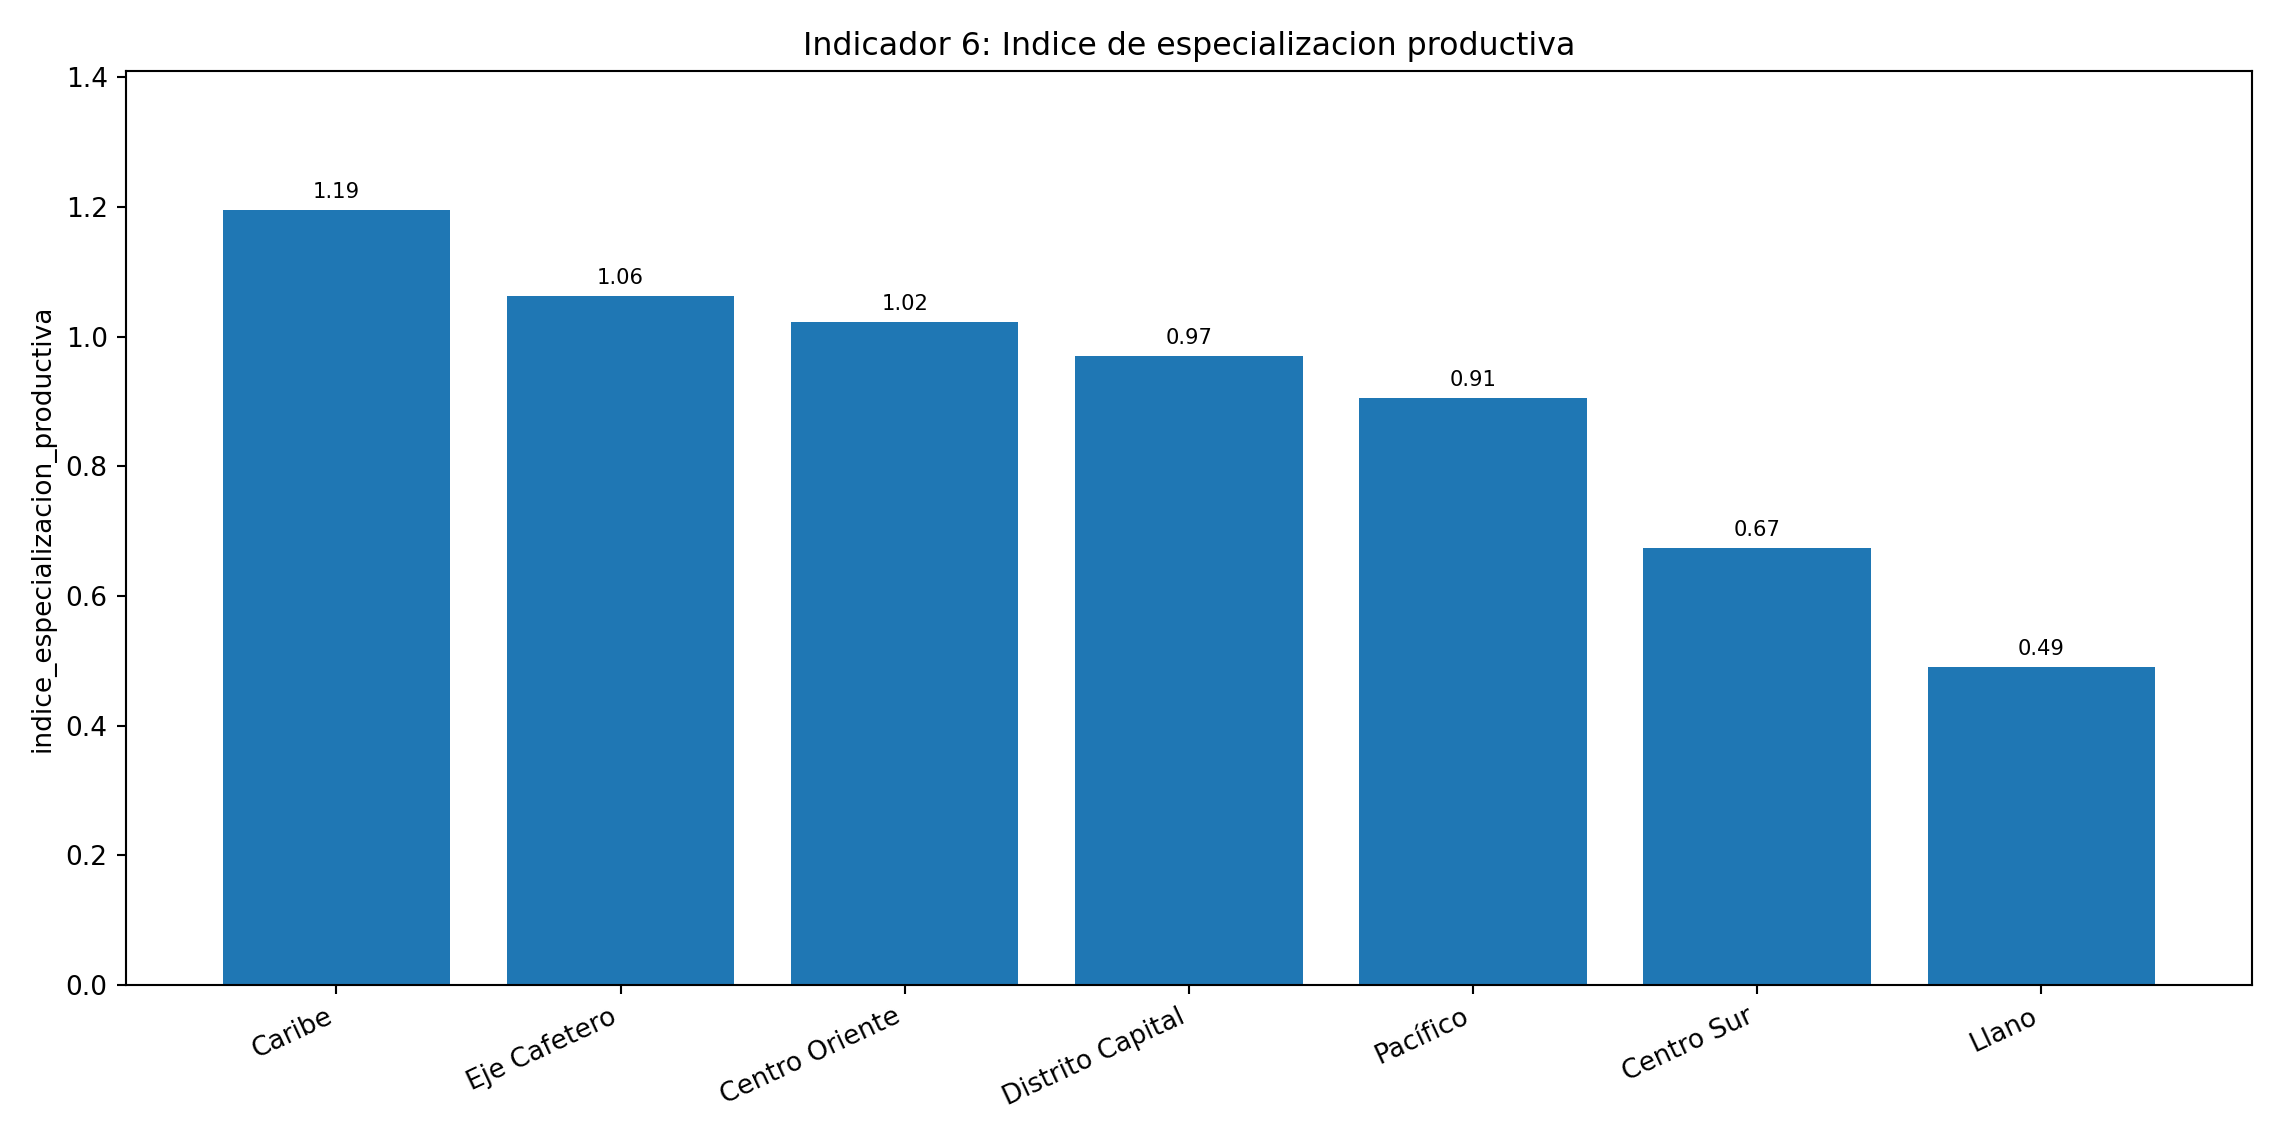
\includegraphics[width=0.92\textwidth]{indicadores/indicador_06.png}
\caption{Indicador 6. Indice de especializacion productiva.}
\end{figure}

\textbf{Analisis concreto.} El indice de especializacion productiva es superior a 1 en Caribe (1.1947), Eje Cafetero (1.0632) y Centro Oriente (1.0233), lo que indica que estas regiones producen relativamente mas de lo que representan en numero de grupos. En contraste, Llano obtiene 0.4903, valor que refleja una especializacion menor al peso de su base de grupos. Este indicador es util para detectar regiones con rendimiento productivo proporcionalmente alto o bajo.



\subsection{Indicador 7. Diversidad relativa de productos}
\textbf{Formula:}
\[
DR_r = \frac{\text{tipologias distintas}_r}{\text{tipologias nacionales}} \times 100
\]
\textbf{Para que se utiliza:} comparar el alcance relativo de diversidad regional frente al universo nacional.


\begin{table}[H]
\centering

\caption{Indicador 7. Diversidad relativa (\%) por región}
\label{tab:ind07_general}

\begin{tabular}{lrrrr}
\toprule
\textbf{Región} & 
\textbf{Tipologías distintas} & 
\textbf{Productos considerados} & 
\textbf{Total tipologías nacionales} & 
\textbf{Diversidad relativa (\%)} \\
\midrule

Distrito Capital & 75 & 413229 & 76 & 98.6842 \\
Eje Cafetero & 74 & 277698 & 76 & 97.3684 \\
Centro Oriente & 71 & 168798 & 76 & 93.4211 \\
Pacífico & 71 & 136445 & 76 & 93.4211 \\
Caribe & 70 & 201994 & 76 & 92.1053 \\
Centro Sur & 66 & 31972 & 76 & 86.8421 \\
Llano & 59 & 10714 & 76 & 77.6316 \\

\bottomrule
\end{tabular}

\end{table}



\begin{figure}[H]
\centering
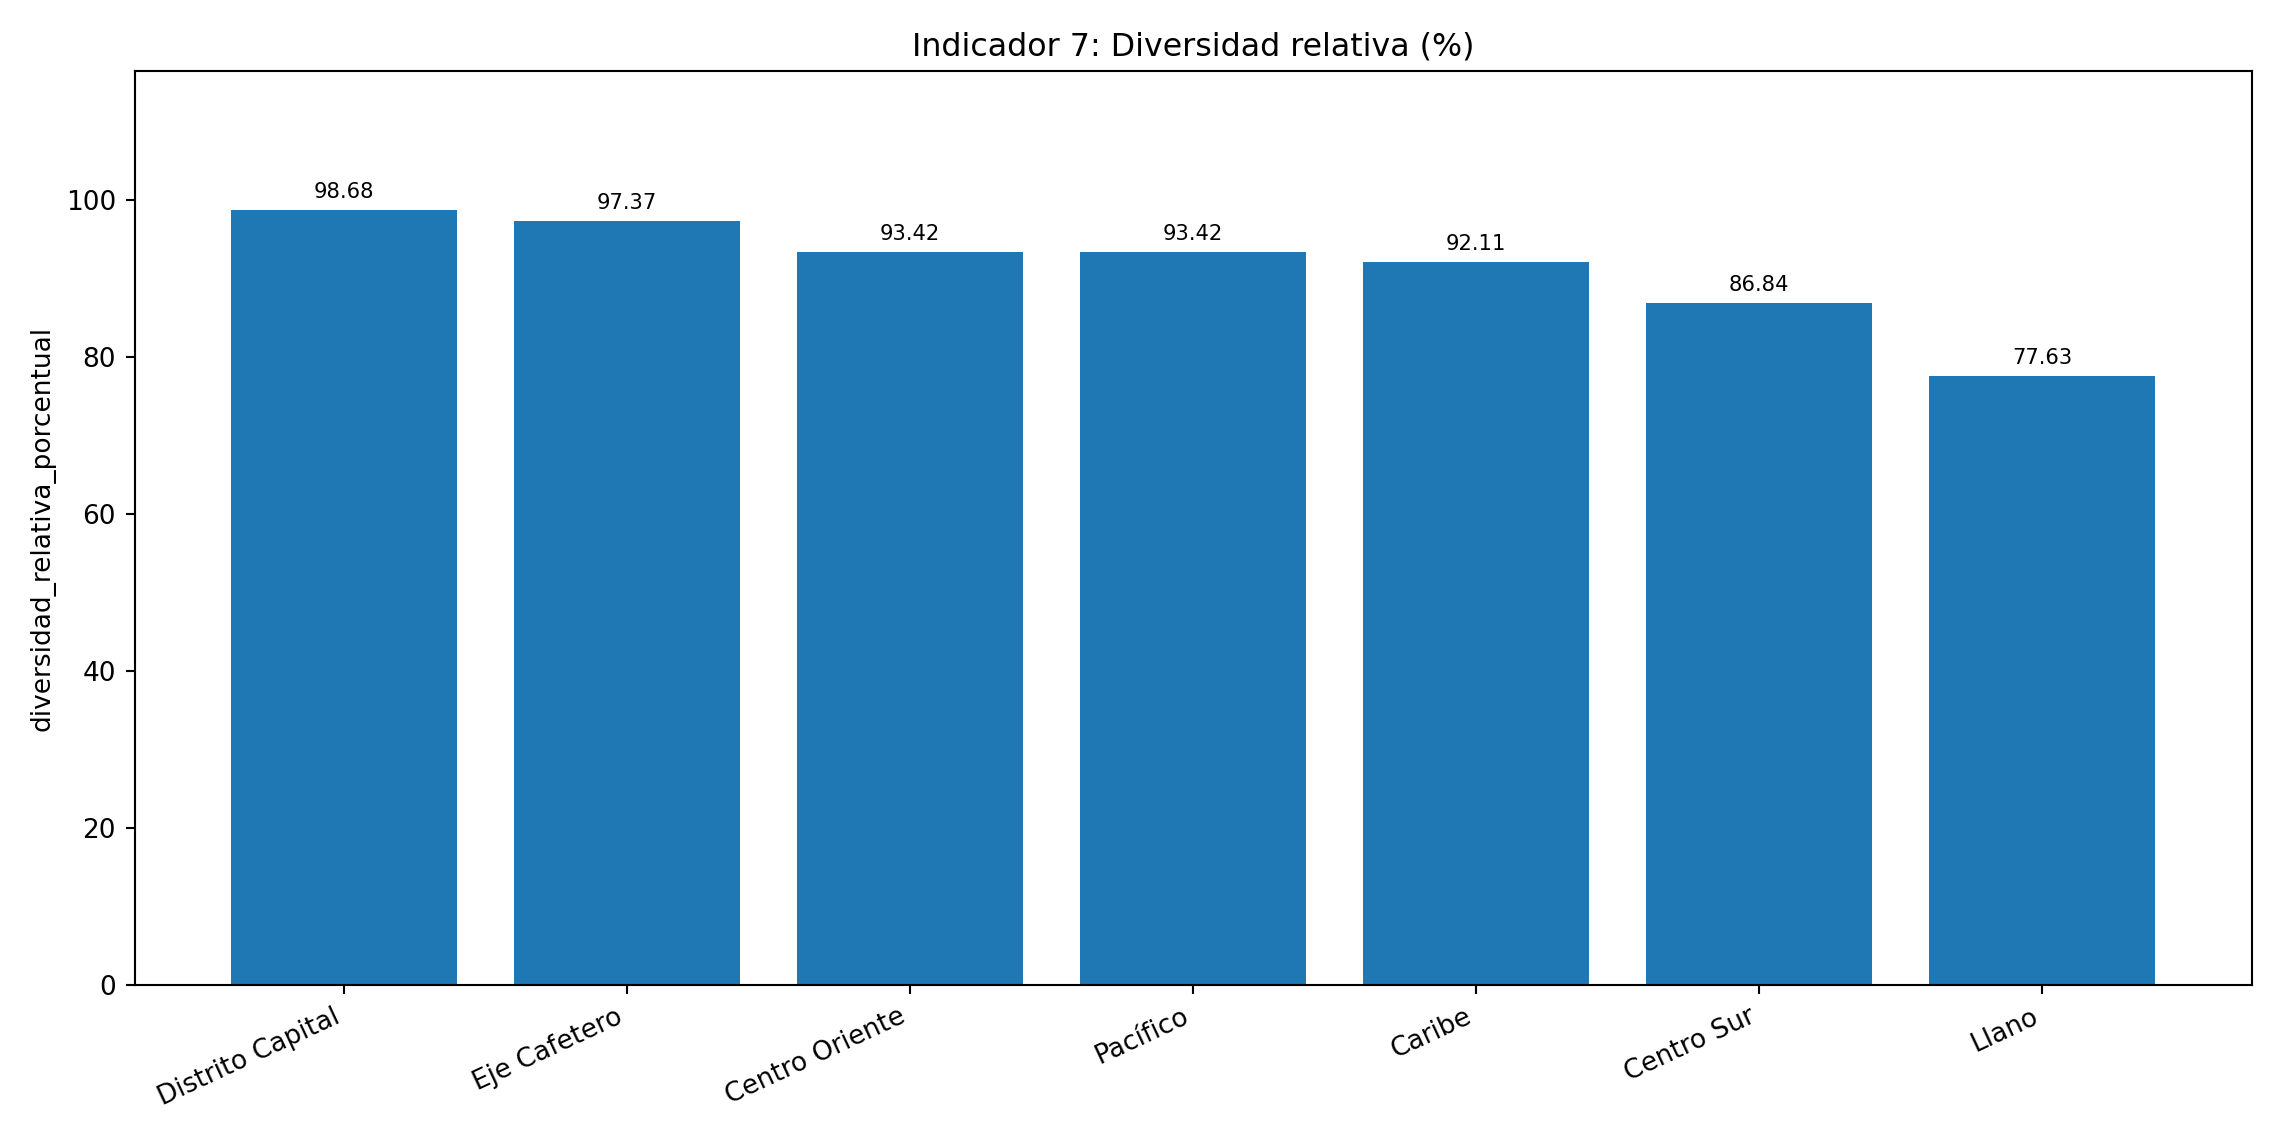
\includegraphics[width=0.92\textwidth]{indicadores/indicador_07.png}
\caption{Indicador 7. Diversidad relativa de productos.}
\end{figure}

\textbf{Analisis concreto.} La diversidad relativa muestra un patron de alta cobertura en Distrito Capital (98.6842\%) y Eje Cafetero (97.3684\%), muy cercanos al maximo teorico de 100\%. En contraste, Llano registra 77.6316\%, lo que evidencia una canasta de tipologias mas concentrada. En terminos estadisticos, la brecha entre maximo y minimo (21.0526 p.p.) confirma heterogeneidad territorial en amplitud de produccion.

\subsection{Indicador 8. Tasa de permanencia de grupos}
\textbf{Formula:}
\[
TP_r = \frac{\text{grupos presentes en 2017, 2019 y 2021}}{\text{grupos unicos}_r} \times 100
\]
\textbf{Para que se utiliza:} medir estabilidad temporal de grupos por region.

\begin{table}[H]
\centering

\caption{Indicador 8. Tasa de permanencia de grupos (\%) por región}
\label{tab:ind08_general}

\begin{tabular}{lrrr}
\toprule
\textbf{Región} & 
\textbf{Grupos únicos} & 
\textbf{Grupos permanentes} & 
\textbf{Tasa de permanencia (\%)} \\
\midrule

Caribe & 859 & 578 & 67.2875 \\
Eje Cafetero & 1327 & 862 & 64.9586 \\
Distrito Capital & 2163 & 1328 & 61.3962 \\
Centro Oriente & 838 & 501 & 59.7852 \\
Pacífico & 765 & 455 & 59.4771 \\
Centro Sur & 241 & 123 & 51.0373 \\
Llano & 111 & 41 & 36.9369 \\

\bottomrule
\end{tabular}

\end{table}


\begin{figure}[H]
\centering
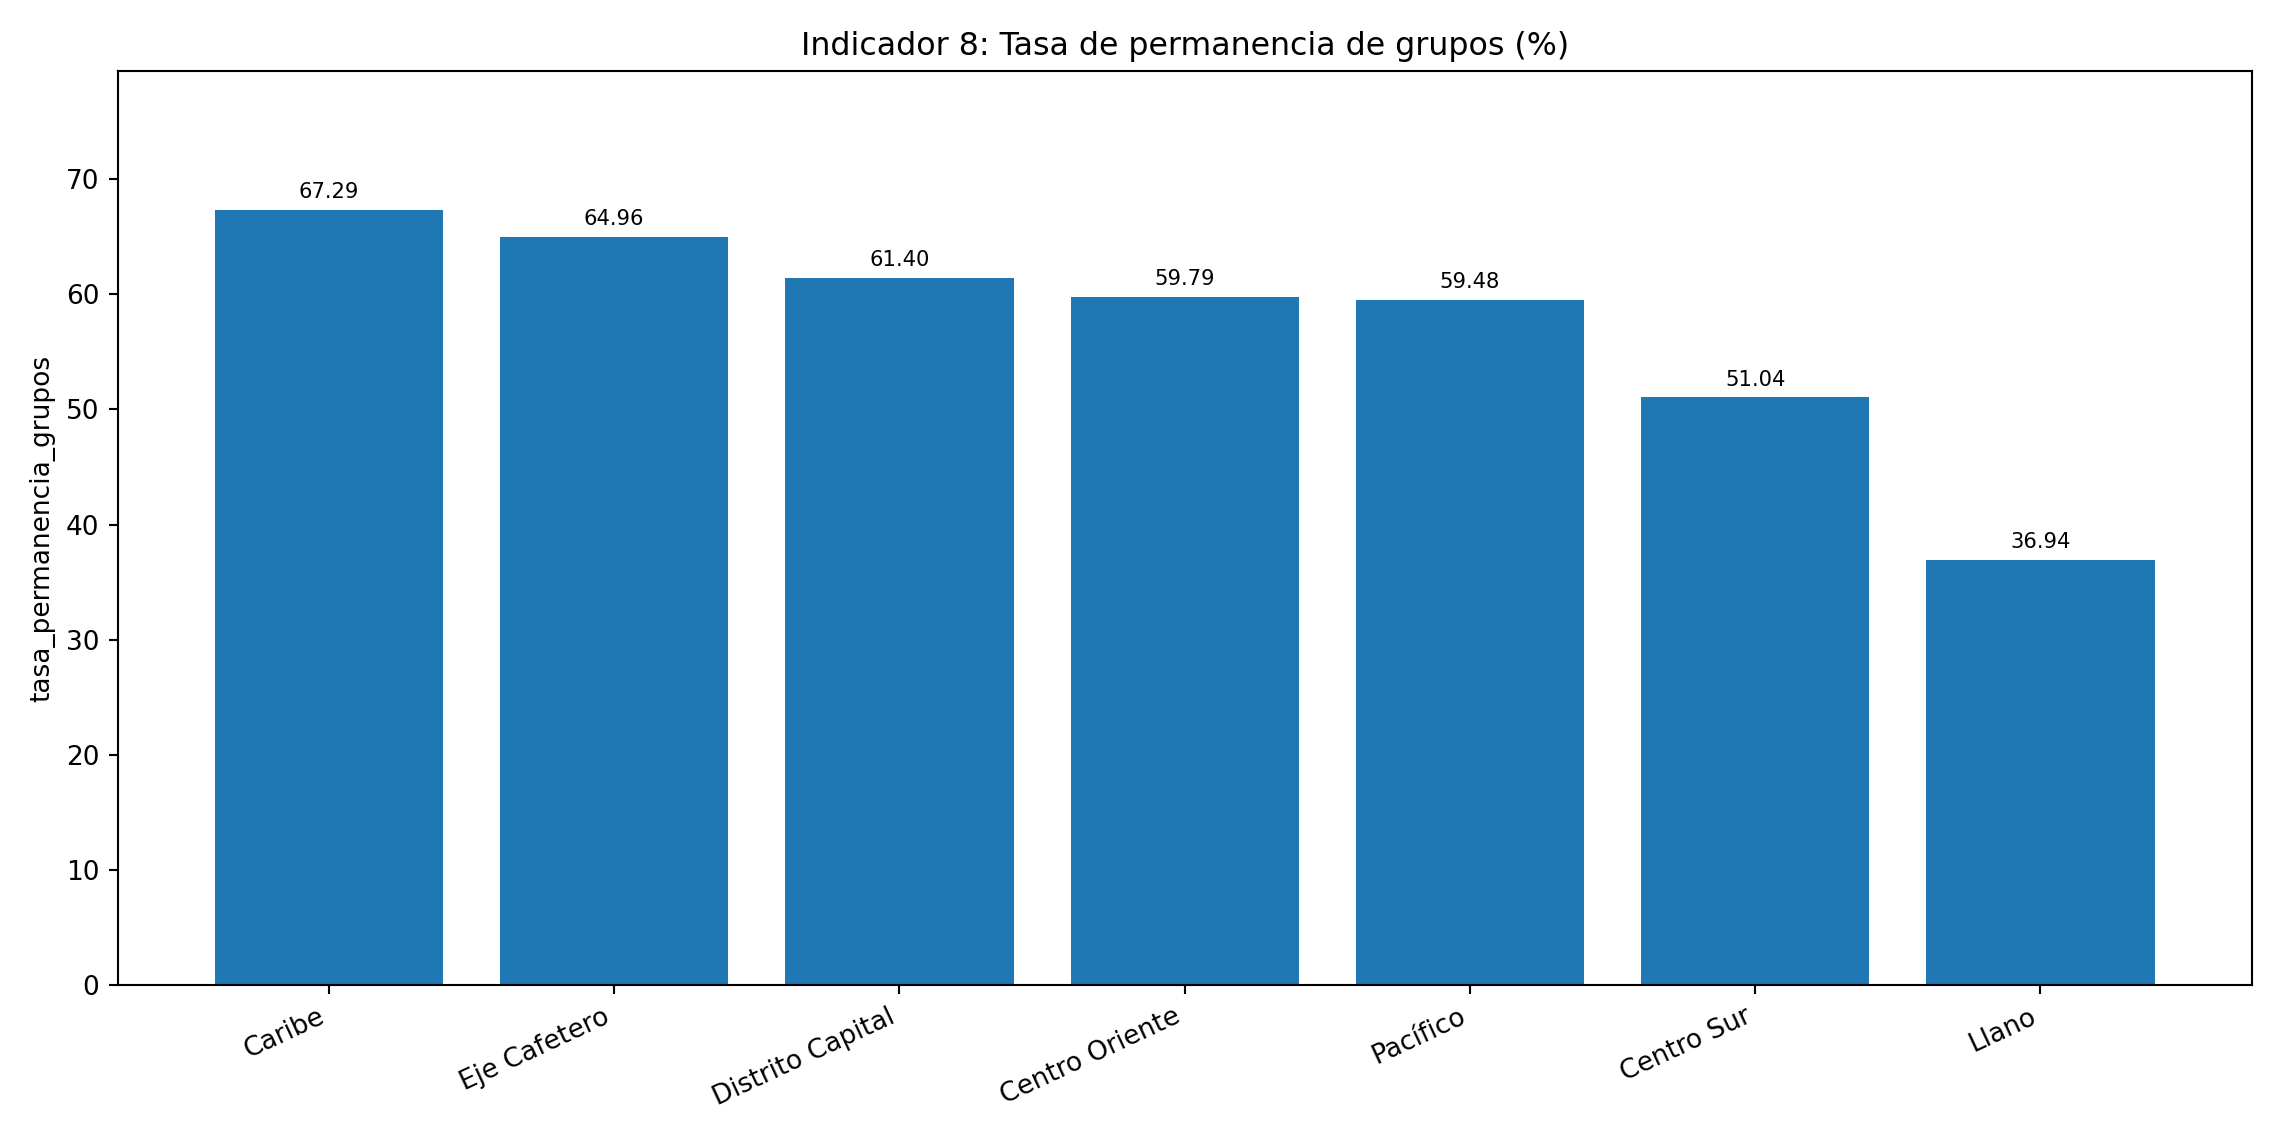
\includegraphics[width=0.92\textwidth]{indicadores/indicador_08.png}
\caption{Indicador 8. Tasa de permanencia de grupos.}
\end{figure}

\textbf{Analisis concreto.} La permanencia de grupos es mas alta en Caribe (67.2875\%) y Eje Cafetero (64.9586\%), indicando mayor estabilidad interconvocatoria. El valor mas bajo corresponde a Llano (36.9369\%), lo que sugiere mayor rotacion estructural de grupos. Esta diferencia de 30.3506 p.p. entre extremos indica que la persistencia institucional no es homogenea entre regiones.

\subsection{Indicador 9. Crecimiento neto de grupos 2017-2021}
\textbf{Formula:}
\[
C_r = \frac{G_{2021} - G_{2017}}{G_{2017}} \times 100
\]
\textbf{Para que se utiliza:} cuantificar crecimiento o disminucion relativa de grupos en el periodo.

\begin{table}[H]
\centering

\caption{Indicador 9. Crecimiento neto de grupos 2017--2021 (\%) por región}
\label{tab:ind09_general}

\begin{tabular}{lrrrrr}
\toprule
\textbf{Región} & 
\textbf{Grupos 2017} & 
\textbf{Grupos 2019} & 
\textbf{Grupos 2021} & 
\textbf{Crecimiento neto} & 
\textbf{Crecimiento porcentual (\%)} \\
\midrule

Llano & 55 & 83 & 93 & 38 & 69.0909 \\
Centro Sur & 154 & 188 & 210 & 56 & 36.3636 \\
Centro Oriente & 569 & 703 & 775 & 206 & 36.2039 \\
Pacífico & 526 & 636 & 688 & 162 & 30.7985 \\
Caribe & 620 & 751 & 810 & 190 & 30.6452 \\
Eje Cafetero & 977 & 1175 & 1206 & 229 & 23.4391 \\
Distrito Capital & 1628 & 1765 & 1855 & 227 & 13.9435 \\

\bottomrule
\end{tabular}

\end{table}

\begin{figure}[H]
\centering
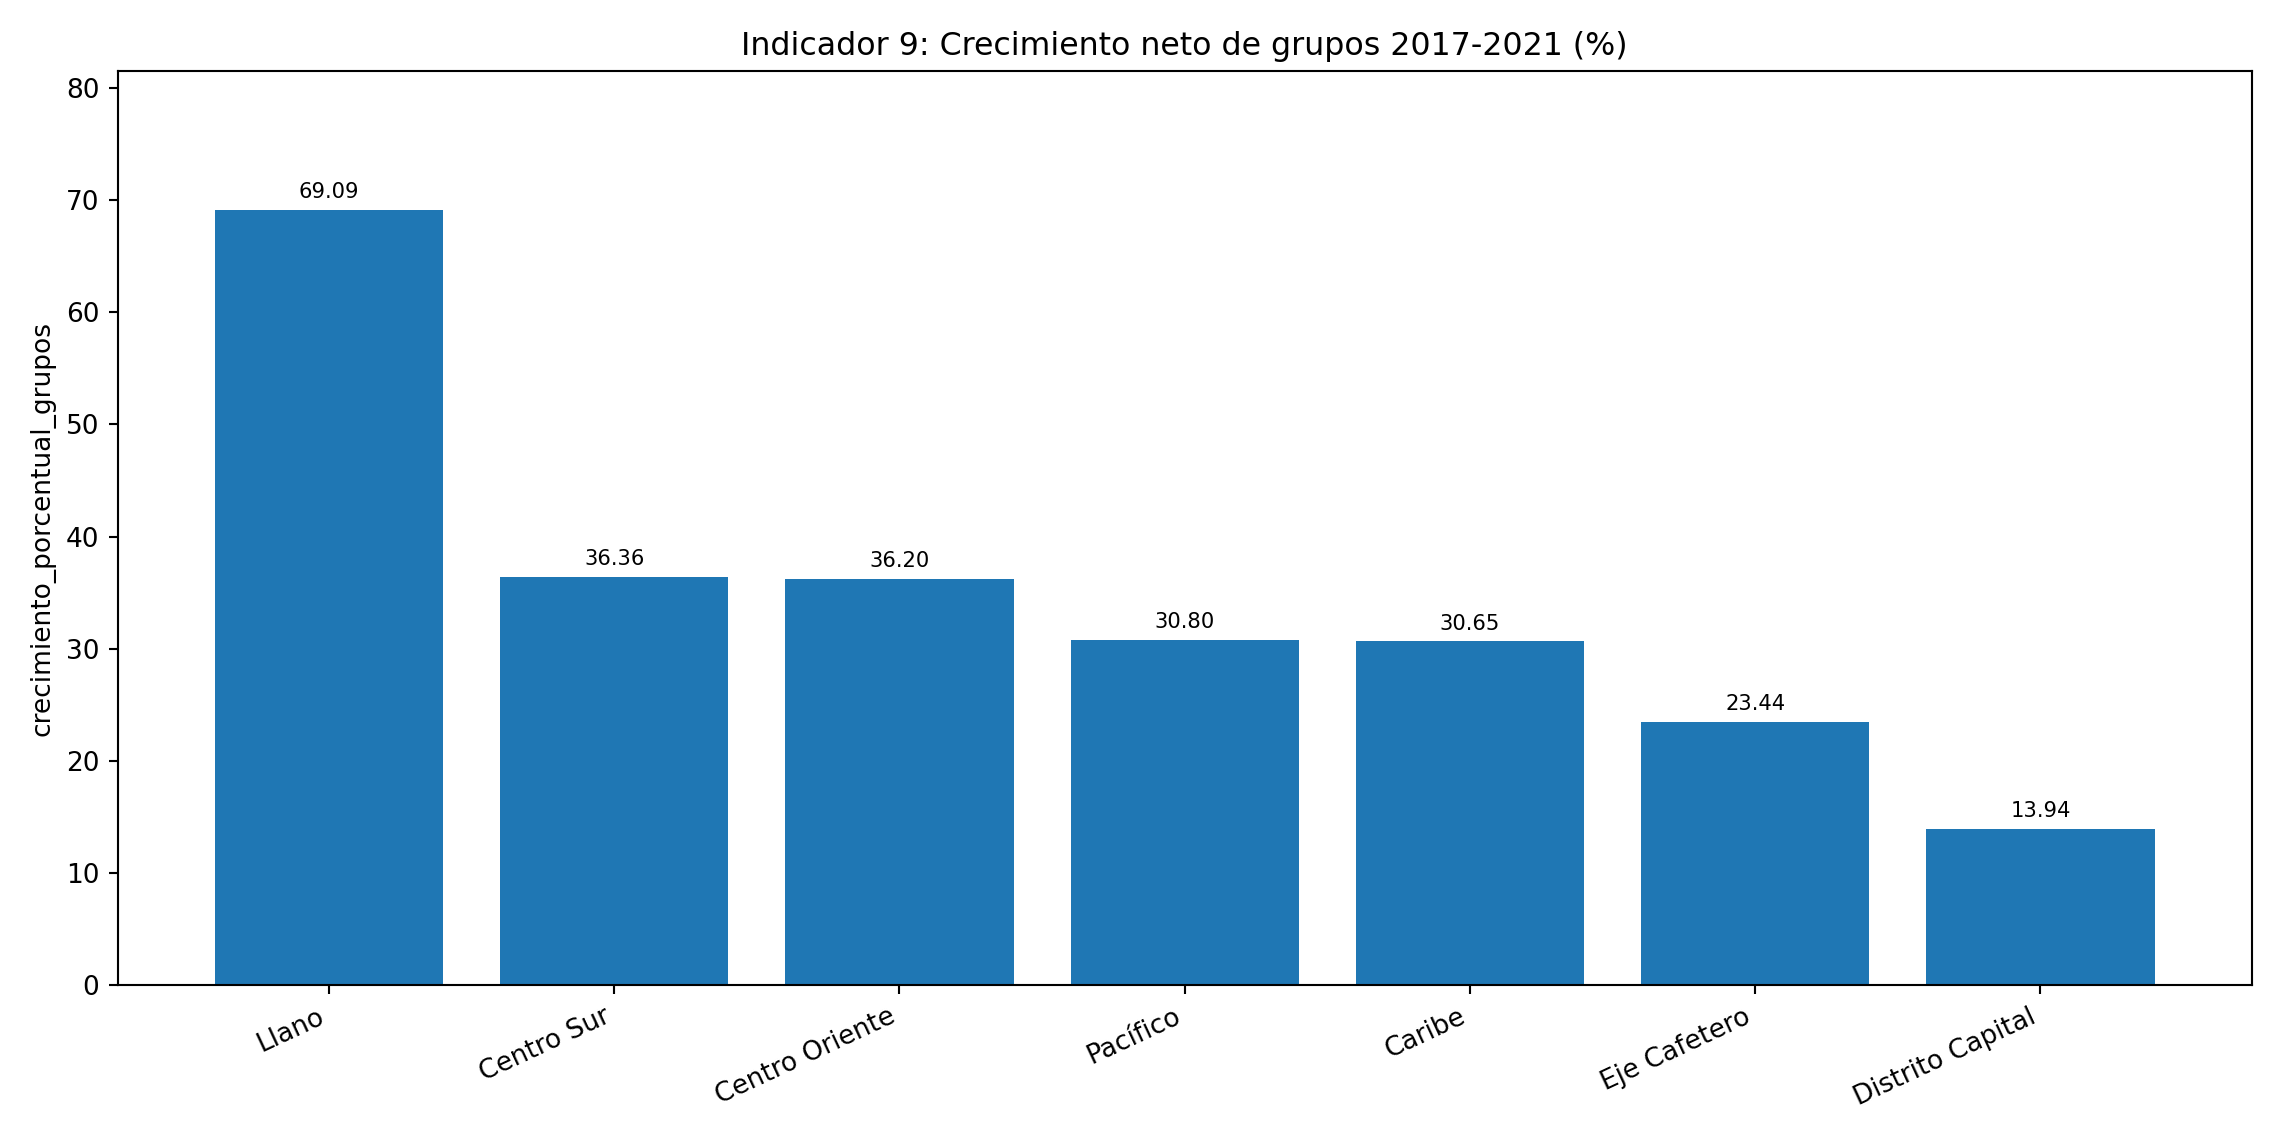
\includegraphics[width=0.92\textwidth]{indicadores/indicador_09.png}
\caption{Indicador 9. Crecimiento neto de grupos 2017-2021.}
\end{figure}

\textbf{Analisis concreto.} El crecimiento neto 2017-2021 es claramente liderado por Llano (69.0909\%), seguido por Centro Sur (36.3636\%). Distrito Capital presenta el menor crecimiento porcentual (13.9435\%), consistente con un efecto de base alta. El patron es compatible con convergencia parcial: regiones pequenas crecen mas rapido en terminos relativos, aunque no necesariamente en volumen absoluto.

\subsection{Indicador 10. Fortaleza A1/A en 2021}
\textbf{Formula:}
\[
FA_{r,2021} = \frac{\text{grupos A1 o A en 2021}_r}{\text{grupos clasificados en 2021}_r} \times 100
\]
\textbf{Para que se utiliza:} medir la fortaleza relativa de clasificaciones altas en 2021.


\begin{table}[H]
\centering

\caption{Indicador 10. Fortaleza A1/A en 2021 (\%) por región}
\label{tab:ind10_general}

\resizebox{\textwidth}{!}{
\begin{tabular}{lrrrr}
\toprule

\textbf{Región} &
\textbf{Grupos clasificados 2021} &
\textbf{Grupos A1/A 2021} &
\textbf{Tasa consolidación A1/A (\%)} &
\textbf{Fortaleza A1/A (\%)} \\

\midrule

Eje Cafetero & 1206 & 538 & 44.6103 & 44.6103 \\
Distrito Capital & 1855 & 677 & 36.4960 & 36.4960 \\
Caribe & 810 & 289 & 35.6790 & 35.6790 \\
Pacífico & 688 & 221 & 32.1221 & 32.1221 \\
Centro Oriente & 775 & 223 & 28.7742 & 28.7742 \\
Centro Sur & 210 & 42 & 20.0000 & 20.0000 \\
Llano & 93 & 7 & 7.5269 & 7.5269 \\

\bottomrule
\end{tabular}
}

\end{table}


\begin{figure}[H]
\centering
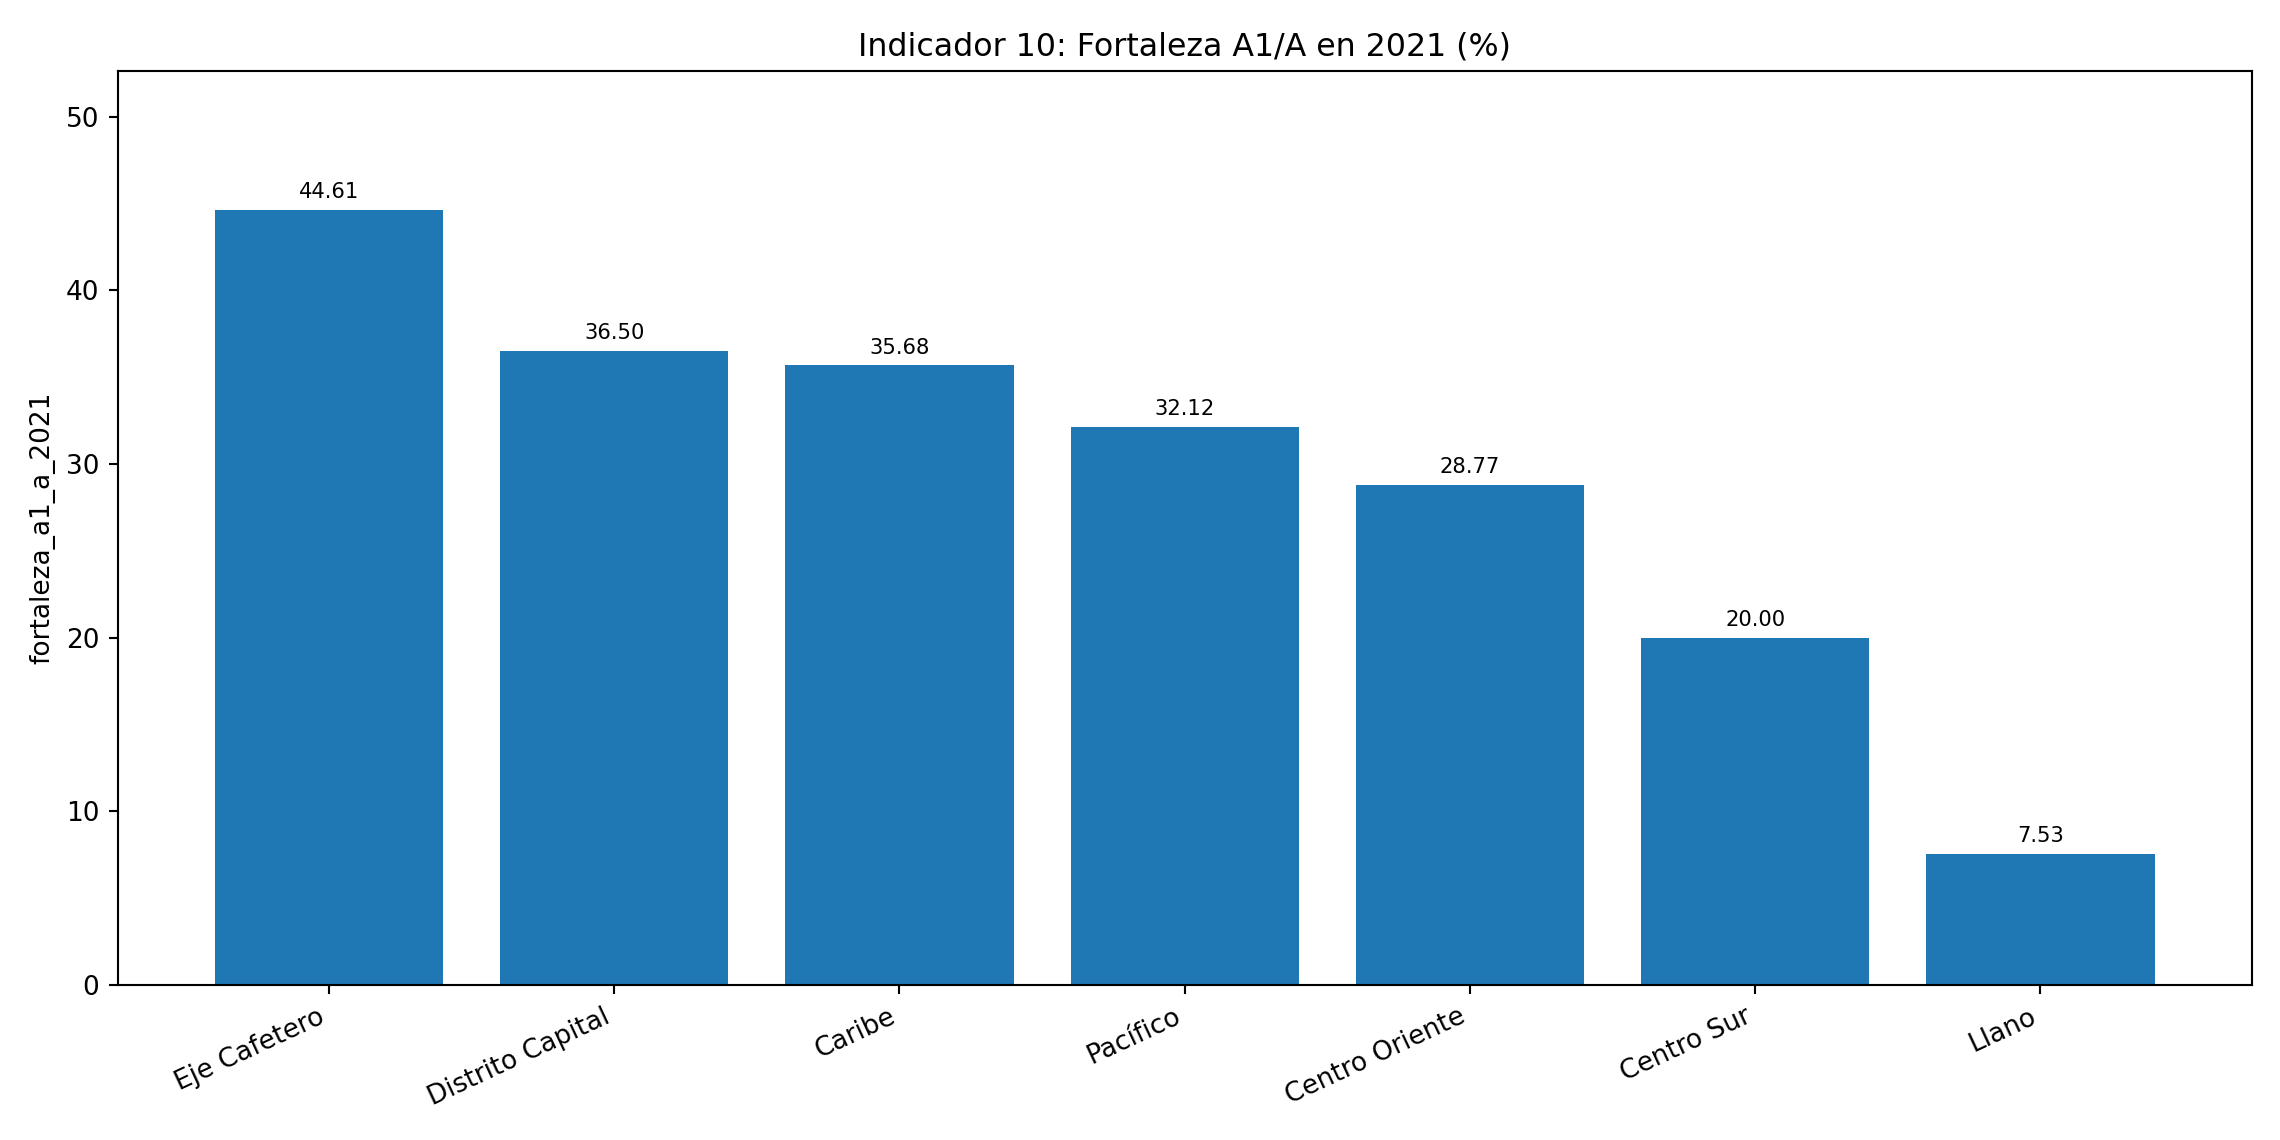
\includegraphics[width=0.92\textwidth]{indicadores/indicador_10.png}
\caption{Indicador 10. Fortaleza A1/A en 2021.}
\end{figure}

\textbf{Analisis concreto.} La fortaleza A1/A en 2021 ubica a Eje Cafetero como lider (44.6103\%), seguido de Distrito Capital (36.4960\%). Llano se encuentra en el minimo (7.5269\%), mostrando una composicion con menor peso de categorias de excelencia. La amplitud entre maximo y minimo (37.0834 p.p.) respalda la existencia de brechas de consolidacion cientifica entre regiones.

\subsection{Indicador 11. Tasa de renovacion de grupos}
\textbf{Formula:}
\[
TR_r = \frac{\text{grupos en 2021 que no estaban en 2017}}{\text{grupos de 2021}_r} \times 100
\]
\textbf{Para que se utiliza:} evaluar la entrada de grupos nuevos entre el inicio y fin del periodo.


\begin{table}[H]
\centering

\caption{Indicador 11. Tasa de renovación de grupos (\%) por región}
\label{tab:ind11_general}

\resizebox{\textwidth}{!}{
\begin{tabular}{lrrr}

\toprule

\textbf{Región} & 
\textbf{Grupos 2021} & 
\textbf{Grupos nuevos 2021 vs 2017} & 
\textbf{Tasa de renovación (\%)} \\

\midrule

Llano & 93 & 50 & 53.7634 \\
Centro Sur & 210 & 80 & 38.0952 \\
Centro Oriente & 775 & 253 & 32.6452 \\
Pacífico & 688 & 216 & 31.3953 \\
Caribe & 810 & 223 & 27.5309 \\
Eje Cafetero & 1206 & 319 & 26.4511 \\
Distrito Capital & 1855 & 481 & 25.9299 \\

\bottomrule

\end{tabular}
}

\end{table}


\begin{figure}[H]
\centering
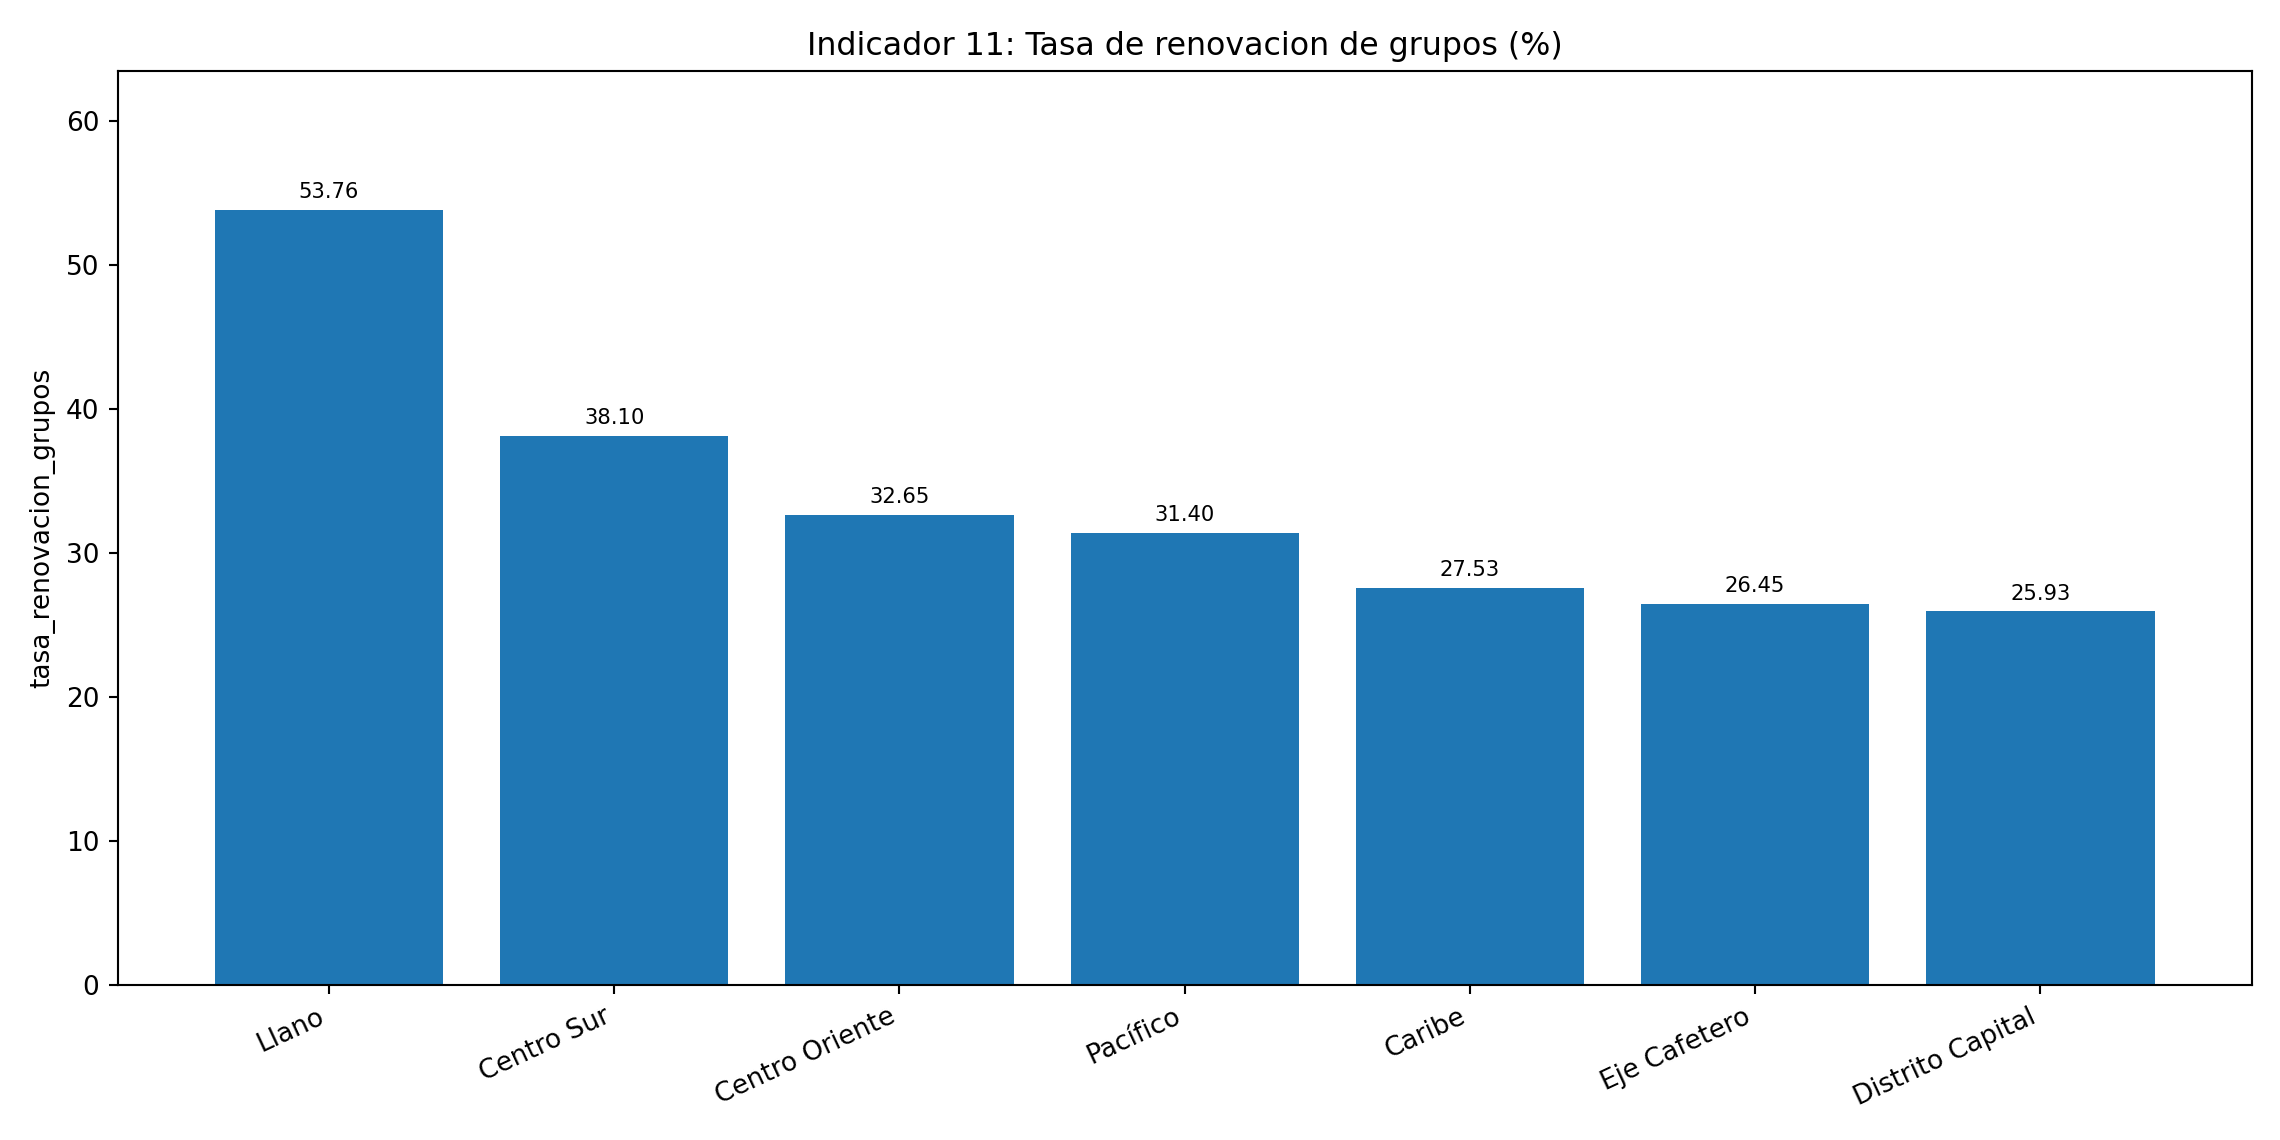
\includegraphics[width=0.92\textwidth]{indicadores/indicador_11.png}
\caption{Indicador 11. Tasa de renovacion de grupos.}
\end{figure}

\textbf{Analisis concreto.} La renovacion de grupos alcanza su maximo en Llano (53.7634\%), lo que indica una alta entrada de grupos nuevos en 2021 respecto de 2017. Distrito Capital presenta el menor valor (25.9299\%), asociado a una estructura mas consolidada y con mayor continuidad. En lectura comparada, la renovacion parece inversamente relacionada con la madurez del sistema regional.

\subsection{Indicador 12. Distribucion por genero registrado}
\textbf{Formula:}
\[
PG_{r,g} = \frac{P_{r,g}}{P_r} \times 100
\]
\textbf{Para que se utiliza:} caracterizar la composicion de produccion por genero dentro de cada region.

\begin{table}[H]
\centering

\caption{Indicador 12. Distribución por género registrado (\%) por región}
\label{tab:ind12_general}

\resizebox{\textwidth}{!}{
\begin{tabular}{llrrrrr}

\toprule

\textbf{Región} &
\textbf{Género} &
\textbf{Productos} &
\textbf{Investigadores únicos} &
\textbf{Total productos región} &
\textbf{Participación (\%)} &
\textbf{Producción promedio} \\

\midrule

Caribe & Masculino & 118156 & 2283 & 201994 & 58.4948 & 51.7547 \\
Caribe & Femenino & 83786 & 1573 & 201994 & 41.4794 & 53.2651 \\
Caribe & Intersexual & 52 & 1 & 201994 & 0.0257 & 52.0000 \\

Centro Oriente & Masculino & 103042 & 2120 & 168798 & 61.0446 & 48.6047 \\
Centro Oriente & Femenino & 65754 & 1378 & 168798 & 38.9543 & 47.7170 \\
Centro Oriente & Intersexual & 2 & 1 & 168798 & 0.0012 & 2.0000 \\

Centro Sur & Masculino & 19303 & 518 & 31972 & 60.3747 & 37.2645 \\
Centro Sur & Femenino & 12669 & 308 & 31972 & 39.6253 & 41.1331 \\

Distrito Capital & Masculino & 260951 & 5248 & 413184 & 63.1561 & 49.7239 \\
Distrito Capital & Femenino & 152225 & 3403 & 413184 & 36.8419 & 44.7326 \\
Distrito Capital & Intersexual & 8 & 1 & 413184 & 0.0019 & 8.0000 \\

Eje Cafetero & Masculino & 179849 & 3629 & 277698 & 64.7642 & 49.5588 \\
Eje Cafetero & Femenino & 97849 & 2196 & 277698 & 35.2358 & 44.5578 \\

Llano & Masculino & 6673 & 188 & 10714 & 62.2830 & 35.4947 \\
Llano & Femenino & 4040 & 119 & 10714 & 37.7077 & 33.9496 \\
Llano & Intersexual & 1 & 1 & 10714 & 0.0093 & 1.0000 \\

Pacífico & Masculino & 87911 & 1770 & 136441 & 64.4315 & 49.6672 \\
Pacífico & Femenino & 48497 & 1137 & 136441 & 35.5443 & 42.6535 \\
Pacífico & Intersexual & 33 & 3 & 136441 & 0.0242 & 11.0000 \\

\bottomrule

\end{tabular}
}

\end{table}

\begin{figure}[H]
\centering
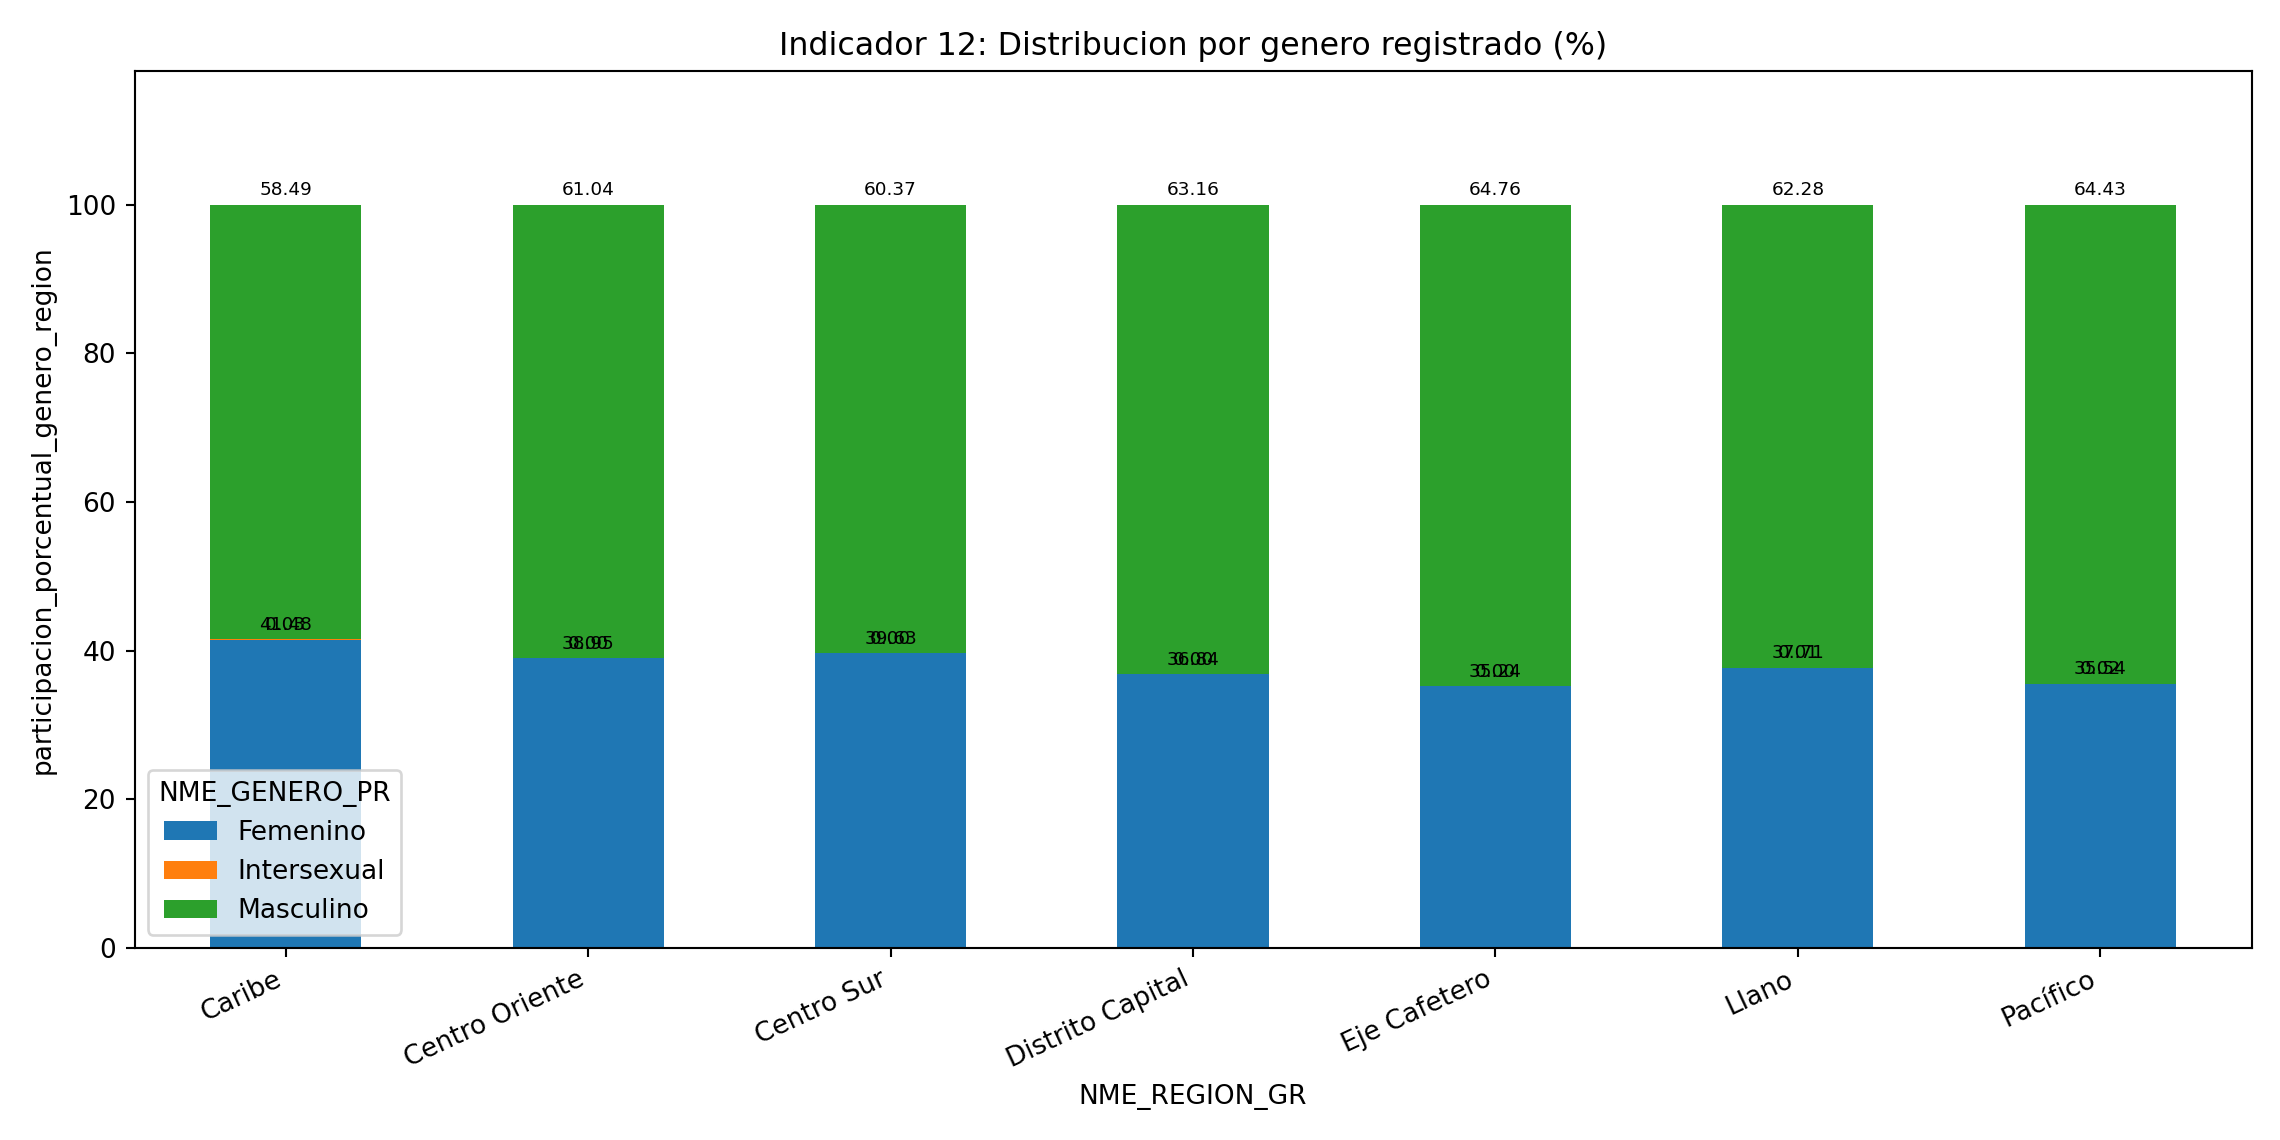
\includegraphics[width=0.92\textwidth]{indicadores/indicador_12.png}
\caption{Indicador 12. Distribucion por genero registrado.}
\end{figure}

\textbf{Analisis concreto.} La distribucion por genero evidencia predominio masculino en todas las regiones analizadas, aunque con magnitudes distintas. La mayor brecha Masculino-Femenino se observa en Eje Cafetero (29.5284 p.p.), mientras Caribe presenta la menor (17.0154 p.p.). Este comportamiento sugiere que la desigualdad de composicion por genero es transversal, pero territorialmente diferenciada.

\subsection{Indicador 13. Evolucion de grupos 2017-2021}
\textbf{Formula:}
\[
E_r = \{\text{nuevos, desaparecen, crecen, decrecen, estables}\}_{2017-2021}
\]
\textbf{Para que se utiliza:} descomponer la dinamica de cambio de grupos por region.


\begin{table}[H]
\centering

\caption{Indicador 13. Evolución de grupos 2017--2021 (\%) por región}
\label{tab:ind13_general}

\resizebox{\textwidth}{!}{
\begin{tabular}{lrrrrrrrrrrrrr}

\toprule

\textbf{Región} &
\textbf{Nuevos} &
\textbf{Desaparecen} &
\textbf{Crecen} &
\textbf{Decrecen} &
\textbf{Estables} &
\textbf{Sin comp.} &
\textbf{Comparables} &
\textbf{Total evolución} &
\textbf{Tasa crecen (\%)} &
\textbf{Tasa decrecen (\%)} &
\textbf{Tasa estabilidad (\%)} &
\textbf{Tasa desaparecen (\%)} &
\textbf{Tasa nuevos (\%)} \\

\midrule

Caribe & 223 & 33 & 449 & 133 & 5 & 16 & 587 & 859 & 76.4906 & 22.6576 & 0.8518 & 3.8417 & 25.9604 \\

Eje Cafetero & 319 & 90 & 675 & 209 & 3 & 31 & 887 & 1327 & 76.0992 & 23.5626 & 0.3382 & 6.7822 & 24.0392 \\

Centro Oriente & 253 & 47 & 397 & 118 & 7 & 16 & 522 & 838 & 76.0536 & 22.6054 & 1.3410 & 5.6086 & 30.1909 \\

Llano & 50 & 12 & 32 & 11 & 0 & 6 & 43 & 111 & 74.4186 & 25.5814 & 0.0000 & 10.8108 & 45.0450 \\

Centro Sur & 80 & 24 & 95 & 33 & 2 & 7 & 130 & 241 & 73.0769 & 25.3846 & 1.5385 & 9.9585 & 33.1950 \\

Distrito Capital & 481 & 254 & 979 & 381 & 14 & 54 & 1374 & 2163 & 71.2518 & 27.7293 & 1.0189 & 11.7429 & 22.2376 \\

Pacífico & 216 & 54 & 311 & 155 & 6 & 23 & 472 & 765 & 65.8898 & 32.8390 & 1.2712 & 7.0588 & 28.2353 \\

\bottomrule

\end{tabular}
}

\end{table}


\begin{figure}[H]
\centering
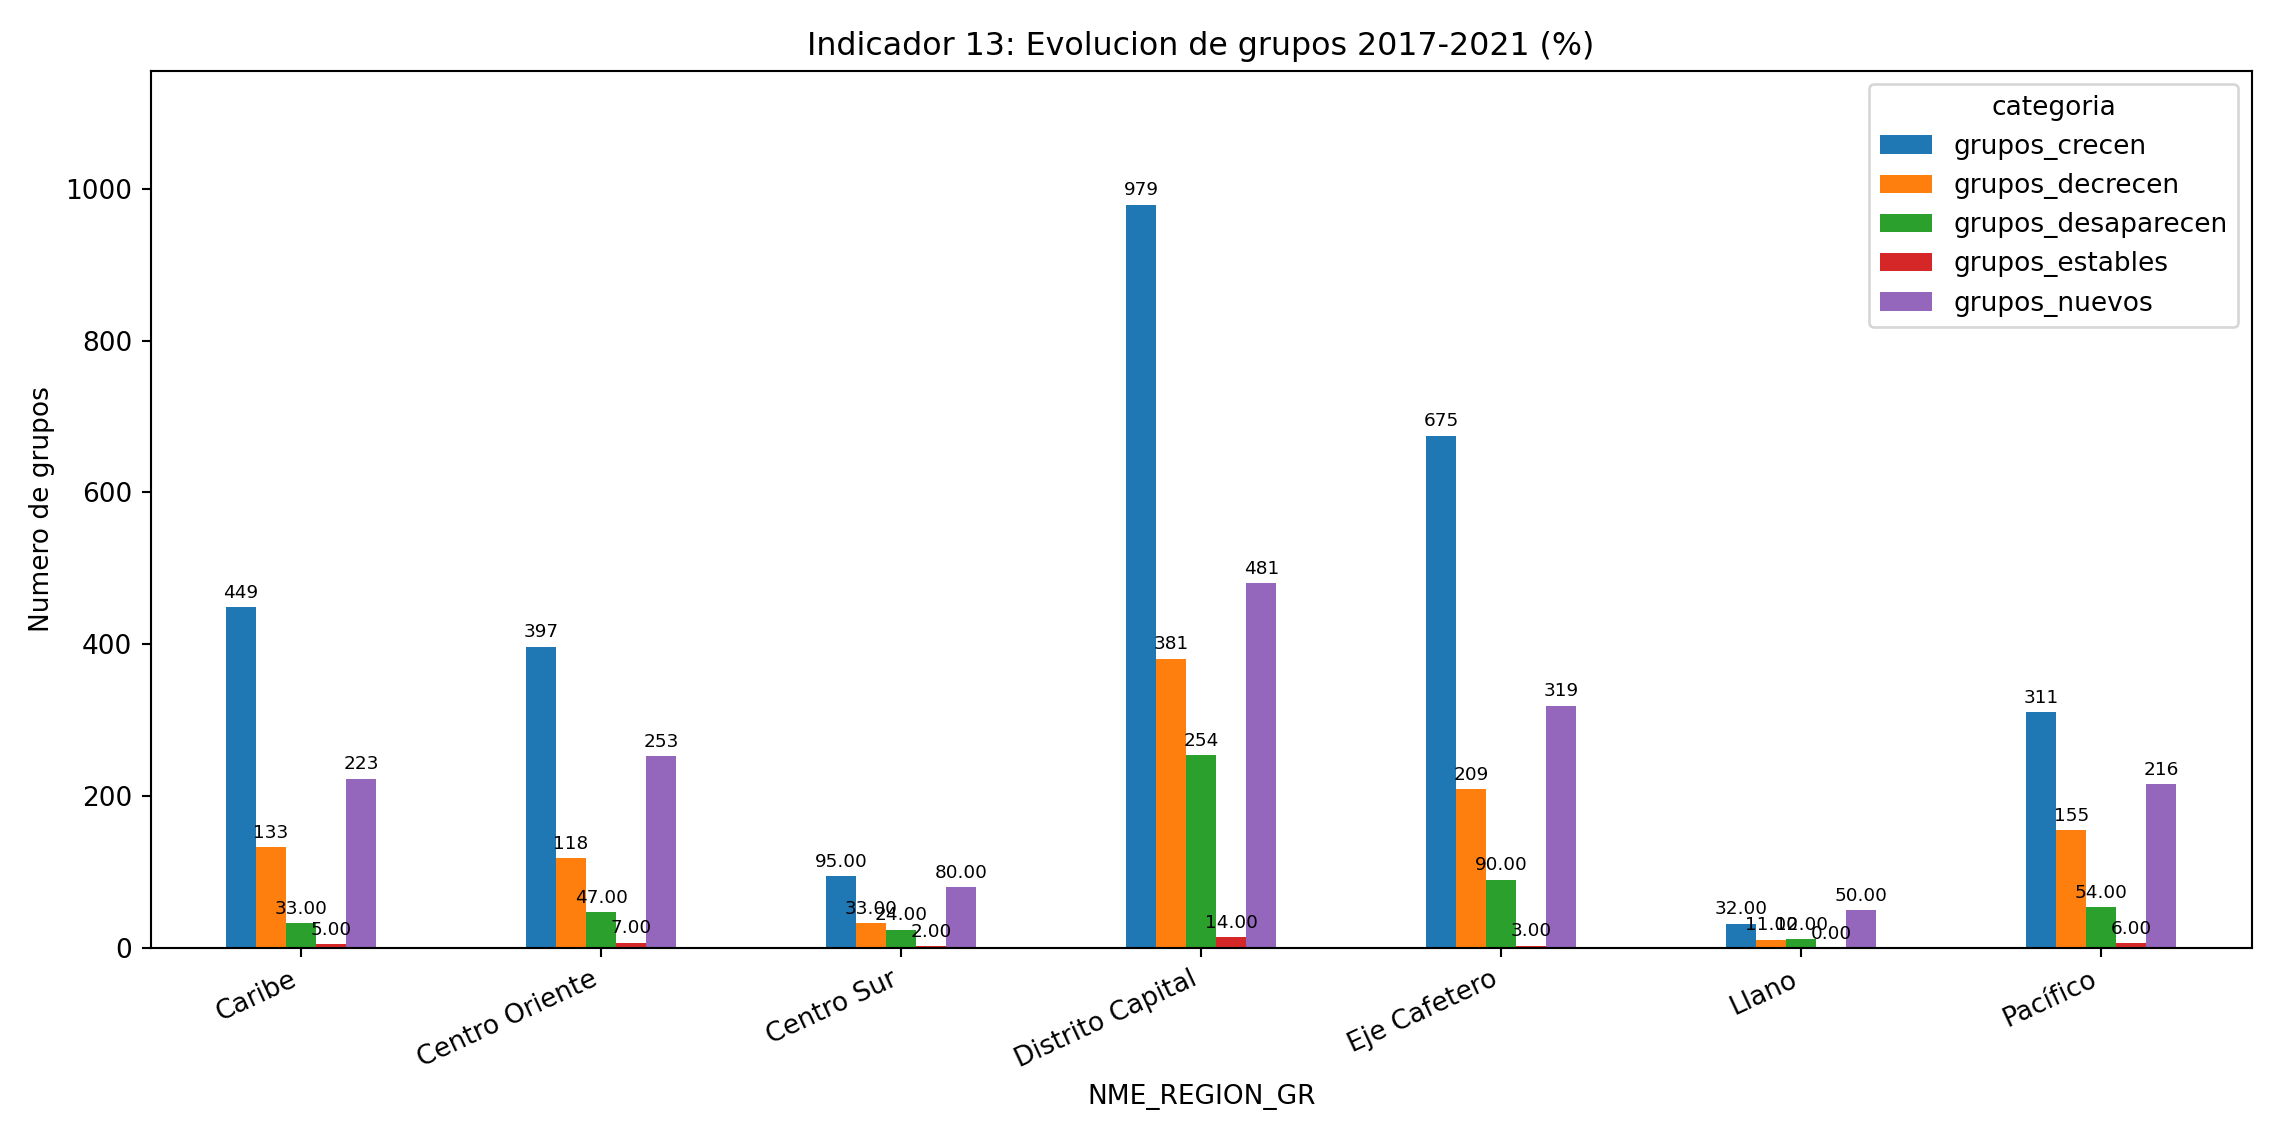
\includegraphics[width=0.92\textwidth]{indicadores/indicador_13.png}
\caption{Indicador 13. Evolucion de grupos 2017-2021.}
\end{figure}

\textbf{Analisis concreto.} En la evolucion 2017-2021 predomina la categoria de grupos que crecen, con maximo en Caribe (76.4906\%) y valores tambien altos en Eje Cafetero. Sin embargo, la dinamica no es unidireccional: Distrito Capital presenta la mayor tasa de desaparicion (11.7429\%), por lo que coexisten expansion y salida de grupos. El resultado sugiere crecimiento neto con recambio interno.

\subsection{Indicador 14. Participacion porcentual por clasificacion del grupo}
\textbf{Formula:}
\[
\%_{r,c} = \frac{P_{r,c}}{P_r} \times 100
\]
\textbf{Para que se utiliza:} comparar composicion interna regional por clasificacion de grupo.

\small

\begin{longtable}{llrrr}

\caption{Indicador 14. Participación por clasificación (\%) por región}
\label{tab:ind14_general} \\

\toprule

\textbf{Región} &
\textbf{Clasificación} &
\textbf{Productos} &
\textbf{Total productos región} &
\textbf{Participación (\%)} \\

\midrule
\endfirsthead

\caption[]{Indicador 14. Participación por clasificación (\%) por región (continuación)} \\

\toprule

\textbf{Región} &
\textbf{Clasificación} &
\textbf{Productos} &
\textbf{Total productos región} &
\textbf{Participación (\%)} \\

\midrule
\endhead

\midrule
\multicolumn{5}{r}{Continúa en la siguiente página} \\
\midrule
\endfoot

\bottomrule
\endlastfoot


Caribe & A & 64347 & 201994 & 31.8559 \\
Caribe & A1 & 52413 & 201994 & 25.9478 \\
Caribe & B & 48907 & 201994 & 24.2121 \\
Caribe & C & 32408 & 201994 & 16.0440 \\
Caribe & Reconocido & 3919 & 201994 & 1.9402 \\

Centro Oriente & A & 49013 & 168798 & 29.0365 \\
Centro Oriente & B & 48710 & 168798 & 28.8570 \\
Centro Oriente & C & 38910 & 168798 & 23.0512 \\
Centro Oriente & A1 & 28675 & 168798 & 16.9878 \\
Centro Oriente & Reconocido & 3490 & 168798 & 2.0676 \\

Centro Sur & B & 9764 & 31972 & 30.5392 \\
Centro Sur & C & 8709 & 31972 & 27.2395 \\
Centro Sur & A & 7579 & 31972 & 23.7051 \\
Centro Sur & A1 & 4275 & 31972 & 13.3711 \\
Centro Sur & Reconocido & 1645 & 31972 & 5.1451 \\

Distrito Capital & A1 & 128489 & 413229 & 31.0939 \\
Distrito Capital & B & 100896 & 413229 & 24.4165 \\
Distrito Capital & A & 98056 & 413229 & 23.7292 \\
Distrito Capital & C & 75452 & 413229 & 18.2591 \\
Distrito Capital & Reconocido & 10336 & 413229 & 2.5013 \\

Eje Cafetero & A1 & 97334 & 277698 & 35.0503 \\
Eje Cafetero & A & 73941 & 277698 & 26.6264 \\
Eje Cafetero & B & 59988 & 277698 & 21.6019 \\
Eje Cafetero & C & 41508 & 277698 & 14.9472 \\
Eje Cafetero & Reconocido & 4927 & 277698 & 1.7742 \\

Llano & C & 5427 & 10714 & 50.6534 \\
Llano & B & 3348 & 10714 & 31.2488 \\
Llano & A & 1190 & 10714 & 11.1070 \\
Llano & A1 & 447 & 10714 & 4.1721 \\
Llano & Reconocido & 302 & 10714 & 2.8187 \\

Pacífico & A1 & 36067 & 136445 & 26.4334 \\
Pacífico & A & 33788 & 136445 & 24.7631 \\
Pacífico & B & 33706 & 136445 & 24.7030 \\
Pacífico & C & 29907 & 136445 & 21.9187 \\
Pacífico & Reconocido & 2977 & 136445 & 2.1818 \\

\end{longtable}

\begin{figure}[H]
\centering
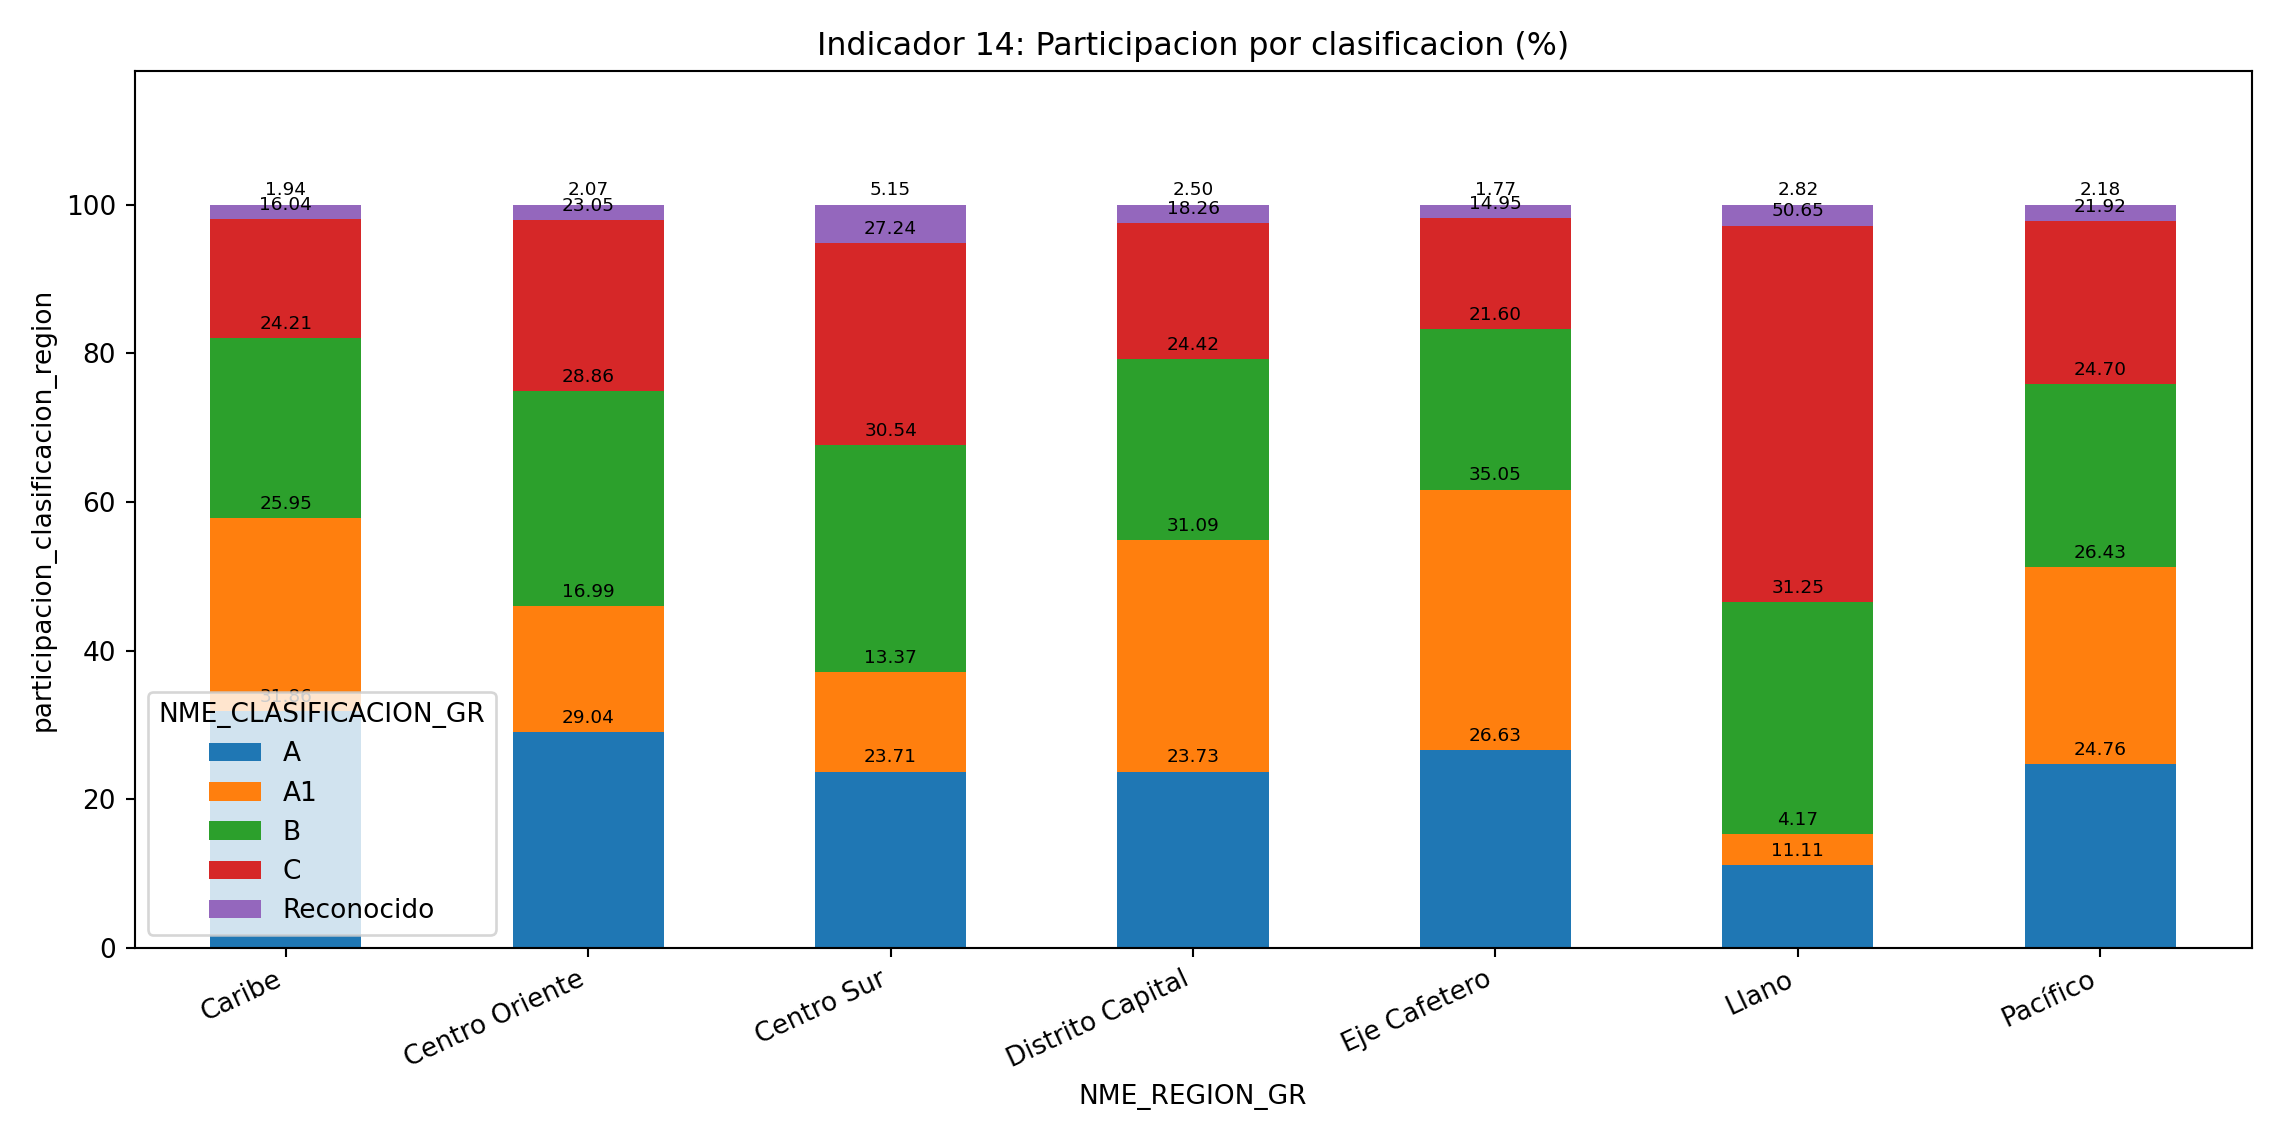
\includegraphics[width=0.92\textwidth]{indicadores/indicador_14.png}
\caption{Indicador 14. Participacion porcentual por clasificacion del grupo.}
\end{figure}

\textbf{Analisis concreto.} La composicion por clasificacion revela perfiles regionales diferenciados: A o A1 lideran en Distrito Capital, Eje Cafetero, Caribe, Centro Oriente y Pacifico; en Centro Sur predomina B; y en Llano domina C (50.6534\%). Esta heterogeneidad estructural confirma que el nivel de madurez cientifica no es uniforme y debe evaluarse con enfoque territorial.

\subsection{Indicador 15. Participacion porcentual por clasificacion, region y convocatoria}
\textbf{Formula:}
\[
\%_{r,c,t} = \frac{P_{r,c,t}}{P_{r,t}} \times 100
\]
\textbf{Para que se utiliza:} analizar cambios de composicion por clasificacion entre convocatorias y regiones.


\small

\begin{longtable}{rrllrrr}

\caption{Indicador 15. Participación por clasificación y convocatoria (\%)}
\label{tab:ind15_conv} \\

\toprule

\textbf{ID} &
\textbf{Año} &
\textbf{Región} &
\textbf{Clasificación} &
\textbf{Productos} &
\textbf{Total región} &
\textbf{Participación (\%)} \\

\midrule
\endfirsthead

\caption[]{Indicador 15. Participación por clasificación y convocatoria (\%) -- continuación} \\

\toprule

\textbf{ID} &
\textbf{Año} &
\textbf{Región} &
\textbf{Clasificación} &
\textbf{Productos} &
\textbf{Total región} &
\textbf{Participación (\%)} \\

\midrule
\endhead

\midrule
\multicolumn{7}{r}{Continúa en la siguiente página} \\
\midrule
\endfoot

\bottomrule
\endlastfoot


19 & 2017 & Caribe & A & 12864 & 40852 & 31.4893 \\
19 & 2017 & Caribe & B & 10471 & 40852 & 25.6315 \\
19 & 2017 & Caribe & A1 & 8510 & 40852 & 20.8313 \\
19 & 2017 & Caribe & C & 8264 & 40852 & 20.2291 \\
19 & 2017 & Caribe & Reconocido & 743 & 40852 & 1.8188 \\

19 & 2017 & Centro Oriente & B & 10738 & 34380 & 31.2333 \\
19 & 2017 & Centro Oriente & C & 8877 & 34380 & 25.8202 \\
19 & 2017 & Centro Oriente & A & 7739 & 34380 & 22.5102 \\
19 & 2017 & Centro Oriente & A1 & 5351 & 34380 & 15.5643 \\
19 & 2017 & Centro Oriente & Reconocido & 1675 & 34380 & 4.8720 \\

19 & 2017 & Centro Sur & C & 1951 & 5953 & 32.7734 \\
19 & 2017 & Centro Sur & B & 1795 & 5953 & 30.1529 \\
19 & 2017 & Centro Sur & A & 1091 & 5953 & 18.3269 \\
19 & 2017 & Centro Sur & A1 & 620 & 5953 & 10.4149 \\
19 & 2017 & Centro Sur & Reconocido & 496 & 5953 & 8.3319 \\

19 & 2017 & Distrito Capital & B & 26502 & 99521 & 26.6296 \\
19 & 2017 & Distrito Capital & A1 & 26289 & 99521 & 26.4155 \\
19 & 2017 & Distrito Capital & C & 22314 & 99521 & 22.4214 \\
19 & 2017 & Distrito Capital & A & 20783 & 99521 & 20.8830 \\
19 & 2017 & Distrito Capital & Reconocido & 3633 & 99521 & 3.6505 \\

19 & 2017 & Eje Cafetero & A1 & 16782 & 57701 & 29.0844 \\
19 & 2017 & Eje Cafetero & B & 15914 & 57701 & 27.5801 \\
19 & 2017 & Eje Cafetero & A & 12867 & 57701 & 22.2994 \\
19 & 2017 & Eje Cafetero & C & 10057 & 57701 & 17.4295 \\
19 & 2017 & Eje Cafetero & Reconocido & 2081 & 57701 & 3.6065 \\

19 & 2017 & Llano & C & 1035 & 1725 & 60.0000 \\
19 & 2017 & Llano & B & 385 & 1725 & 22.3188 \\
19 & 2017 & Llano & A & 162 & 1725 & 9.3913 \\
19 & 2017 & Llano & Reconocido & 143 & 1725 & 8.2899 \\

19 & 2017 & Pacífico & B & 9194 & 31792 & 28.9192 \\
19 & 2017 & Pacífico & A1 & 8781 & 31792 & 27.6202 \\
19 & 2017 & Pacífico & C & 6896 & 31792 & 21.6910 \\
19 & 2017 & Pacífico & A & 6240 & 31792 & 19.6276 \\
19 & 2017 & Pacífico & Reconocido & 681 & 31792 & 2.1420 \\

20 & 2019 & Caribe & A & 24318 & 75971 & 32.0096 \\
20 & 2019 & Caribe & A1 & 19748 & 75971 & 25.9941 \\
20 & 2019 & Caribe & B & 19664 & 75971 & 25.8836 \\
20 & 2019 & Caribe & C & 11494 & 75971 & 15.1295 \\
20 & 2019 & Caribe & Reconocido & 747 & 75971 & 0.9833 \\

% CONTINÚA CON EL RESTO DE FILAS...

\end{longtable}





\begin{figure}[H]
\centering
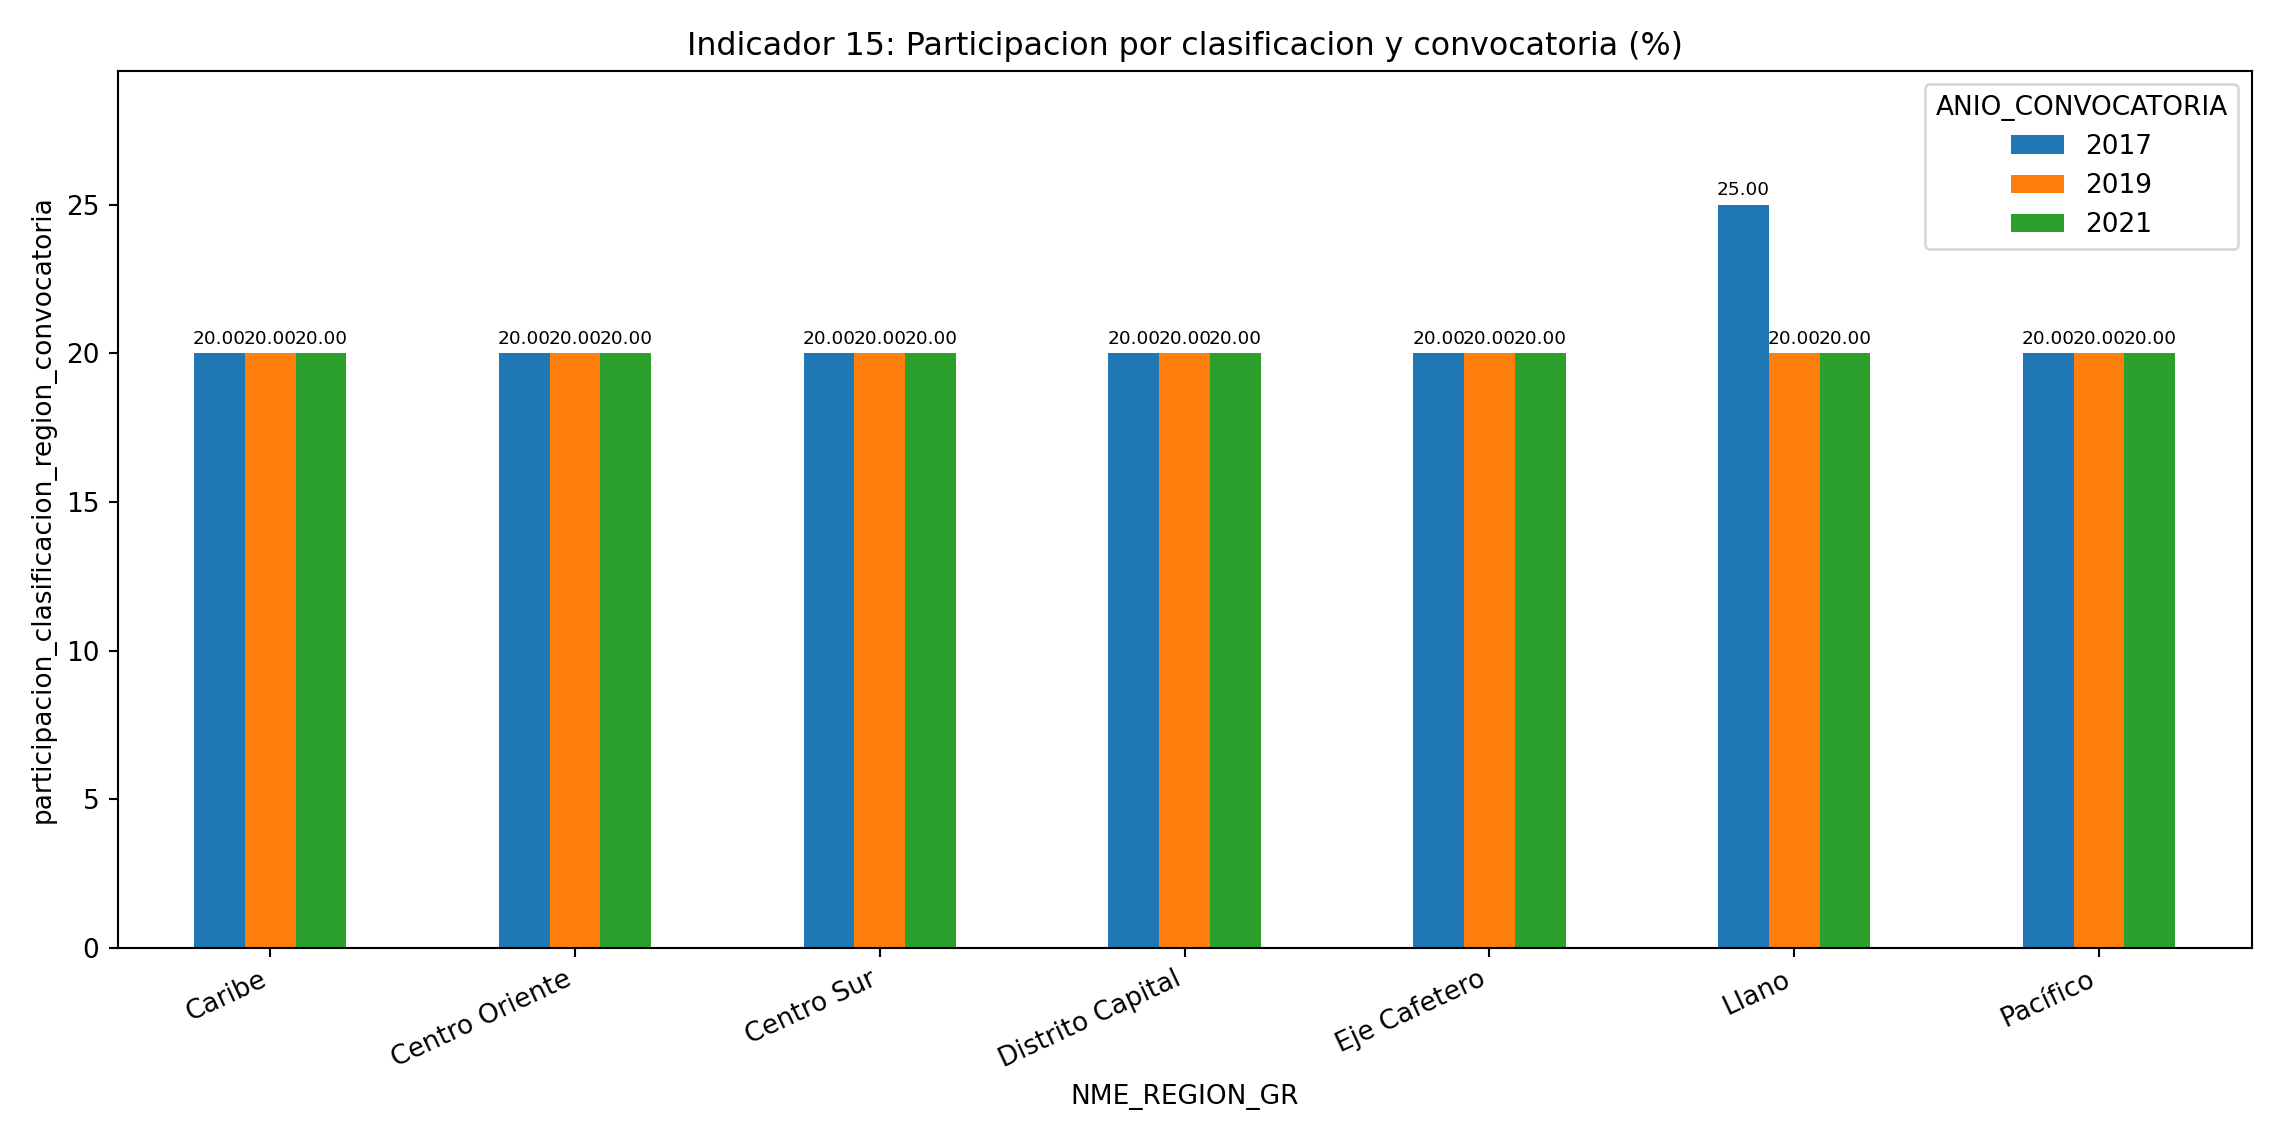
\includegraphics[width=0.92\textwidth]{indicadores/indicador_15.png}
\caption{Indicador 15. Participacion porcentual por clasificacion, region y convocatoria.}
\end{figure}

\textbf{Analisis concreto.} El indicador por clasificacion, region y convocatoria evidencia una tendencia creciente del bloque A1+A entre 2017 y 2021 en todas las regiones. Ejemplos: Eje Cafetero pasa de 51.3838\% a 67.1661\%, Distrito Capital de 47.2985\% a 59.2069\% y Caribe de 52.3206\% a 60.2553\%. Aunque Llano tambien crece (9.3913\% a 17.2052\%), mantiene una estructura con mayor peso relativo de categorias intermedias y bajas.

\section{Discusion}

El conjunto de resultados muestra que la lectura territorial mejora cuando se combinan volumen, estructura y dinamica temporal. Las regiones lideres no coinciden necesariamente en todas las metricas, lo que refuerza la necesidad de una evaluacion multidimensional.

Metodologicamente, el principal aporte fue la integracion entre datos, formulas y visualizacion en un flujo verificable. Esto reduce el riesgo de conclusiones no trazables y facilita la replicacion del analisis.

\section{Conclusiones}

\begin{enumerate}[label=\arabic*.]
  \item Se consolido un proceso reproducible desde datos abiertos hasta producto visual funcional.
  \item Se documentaron 15 indicadores con formula, uso, tabla y grafico, alineados con datos versionados.
  \item El sistema evidencia crecimiento agregado de produccion con patrones de concentracion territorial persistentes.
  \item La comparacion por dimensiones evita lecturas sesgadas basadas en una sola metrica.
\end{enumerate}

\section{Recomendaciones}

\begin{enumerate}[label=\arabic*.]
  \item Mantener actualizacion periodica del pipeline al publicar nuevas convocatorias.
  \item Incorporar analisis de sensibilidad para supuestos de limpieza e integracion.
  \item Extender el tablero con filtros por area de conocimiento y tipo de producto.
\end{enumerate}

\section{Limitaciones}

\begin{itemize}
  \item El analisis depende de la completitud y calidad de los registros abiertos disponibles.
  \item Algunos indicadores estructurales no se desagregan por convocatoria por definicion metodologica.
  \item No se incorporan variables socioeconomicas externas para explicar causalidad territorial.
\end{itemize}

\section{Referencias}

Departamento Administrativo Nacional de Estadistica. (2018). \textit{Censo Nacional de Poblacion y Vivienda 2018}. \url{https://www.dane.gov.co}

Departamento Administrativo Nacional de Estadistica. (2018). \textit{Encuesta Nacional de Calidad de Vida 2018}. \url{https://www.dane.gov.co}

Ministerio de Ciencia, Tecnologia e Innovacion. (s. f.). \textit{Investigadores reconocidos por convocatoria (2017, 2019, 2021)}. Datos Abiertos Colombia. \url{https://www.datos.gov.co/Ciencia-Tecnolog-a-e-Innovaci-n/Investigadores-Reconocidos-por-convocatoria/bqtm-4y2h/about_data}

Ustadistica. (2026). \textit{Observatorio MinCiencias - Investigadores Reconocidos}. GitHub. \url{https://github.com/ustadistica/Observatorio_Ministerio_de_Ciencias_Grupo7}

\end{document}